\noindent

\includegraphics[height=1.25cm]{images/pictograms/benchmark}
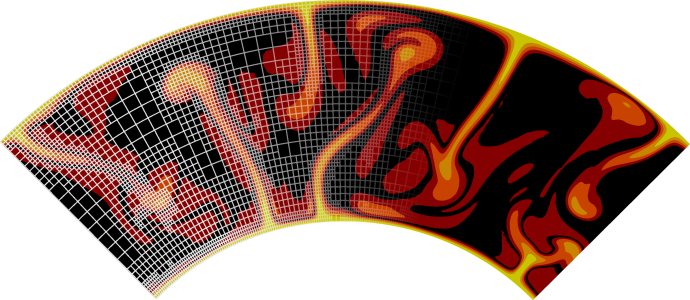
\includegraphics[height=1.25cm]{images/pictograms/aspect_logo}

\includegraphics[height=1.25cm]{images/pictograms/FEM}

\includegraphics[height=1.25cm]{images/pictograms/paraview}


%%%%%%%%%%%%%%%%%%%%%%%%%%%%%%%%%%%%%%%%%%%%%%%%%%%%%%%%%%%%%%%%%%%%%%%%%%%%%%%%%%%%%%%%%%%%%%%%%%%

\begin{flushright} {\tiny {\color{gray} python\_codes/fieldstone\_152/text.tex}} \end{flushright}

\lstinputlisting[language=bash,basicstyle=\small]{python_codes/fieldstone_152/keywords.key}

\par\noindent\rule{\textwidth}{0.4pt}

\begin{center}
\inpython
{\small Code: \url{https://github.com/cedrict/fieldstone/tree/master/python_codes/fieldstone_152}}
\end{center}

\par\noindent\rule{\textwidth}{0.4pt}

%{\sl This stone was developed in collaboration with Donald Duck}. \index{contributors}{D. Duck}

%\par\noindent\rule{\textwidth}{0.4pt}

%%%%%%%%%%%%%%%%%%%%%%%%%%%%%%%%%%%%%%%%%%%%%%%%%%%%%%%%%%%%%%%%%%%%%%%%%%%%%%%%%%%%%%%%%%%%%%%%%%%


The goal here is to explore the influence of the mapping polynomial order and/or
the number of quadrature points on the accuracy of the solution of various benchmarks and test cases.
We will exclusively focus on annulus geometries in plane strain of 
shell geometries by means of an axisymmetric formulation.

Concretely, in this \stone we will explore the effect of:
\begin{itemize}
\item resolution via the number of elements in the radial direction: {\python nelr=2-32} (we automatically set {\python nelt=12*nelr})
\item the number of quadrature points per dimension: {\python nqperdim=2,3,4,5}
\item the polynomial order of the mapping: {\python mapping='Q1','Q2','Q3','Q4'}
\end{itemize}
and we will monitor the computed area/volume, the root mean square velocity and the velocity and pressure errors.

After discretising the domain in {\python nel} elements, and having decided the FE
pair we want to use to solve the Stokes equations (in this case \QtwoQone), we end up 
having to compute elemental integrals such as 
\[
\K_e = \int_{\Omega_e} {\bm B}^T\cdot {\bm C}_\eta \cdot {\bm B} \; d\Omega
\]
where $\Omega_e$ denotes an element.
The way we carry out this integration is by means of the Gauss-Legendre quadrature
(see Section~\ref{MMM-sec:quadrature}), which 
forces us to carry out a change of variables from the original element $\Omega_e$ 
to the reference element $(r,s) \in [-1,1]\times [-1,1]$. For this we establish a mapping between both 
as explained in Section~\ref{MMM-ss:mappings}.
Basis functions $Q_{1,2,3,4}$ are defined in Section~\ref{MMM-sec:shpfct2d}.

\begin{center}
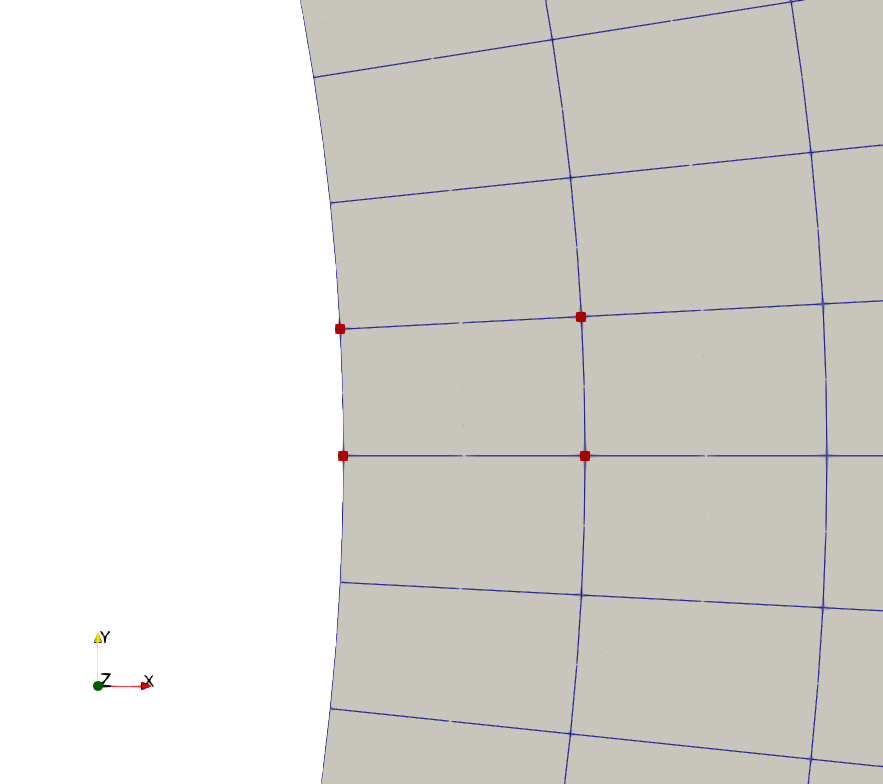
\includegraphics[width=4.2cm]{python_codes/fieldstone_152/images/mappingQ1}
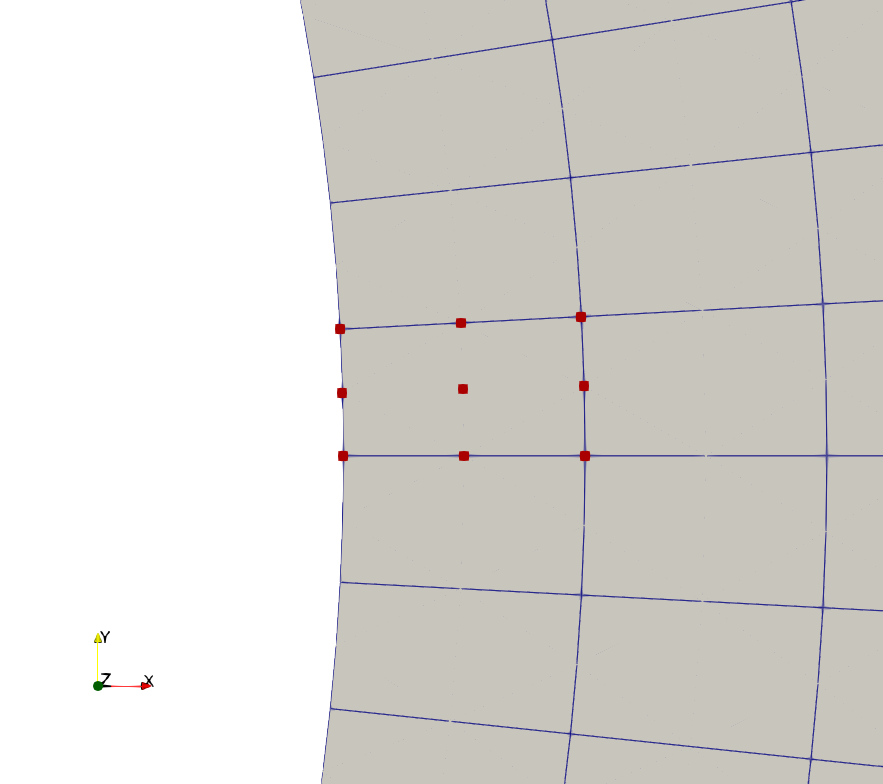
\includegraphics[width=4.2cm]{python_codes/fieldstone_152/images/mappingQ2}
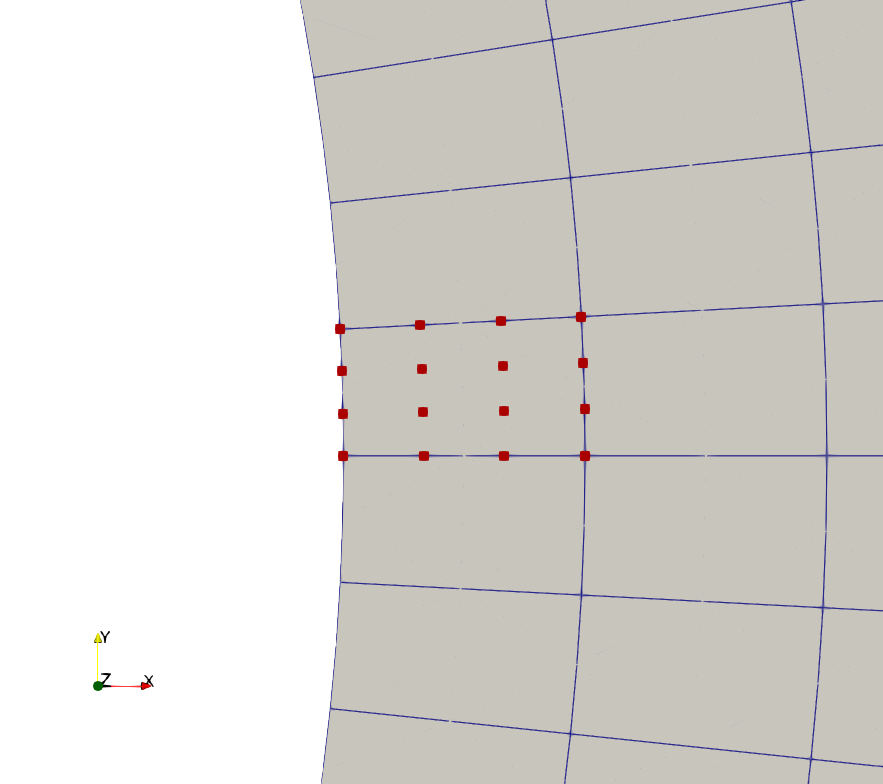
\includegraphics[width=4.2cm]{python_codes/fieldstone_152/images/mappingQ3}
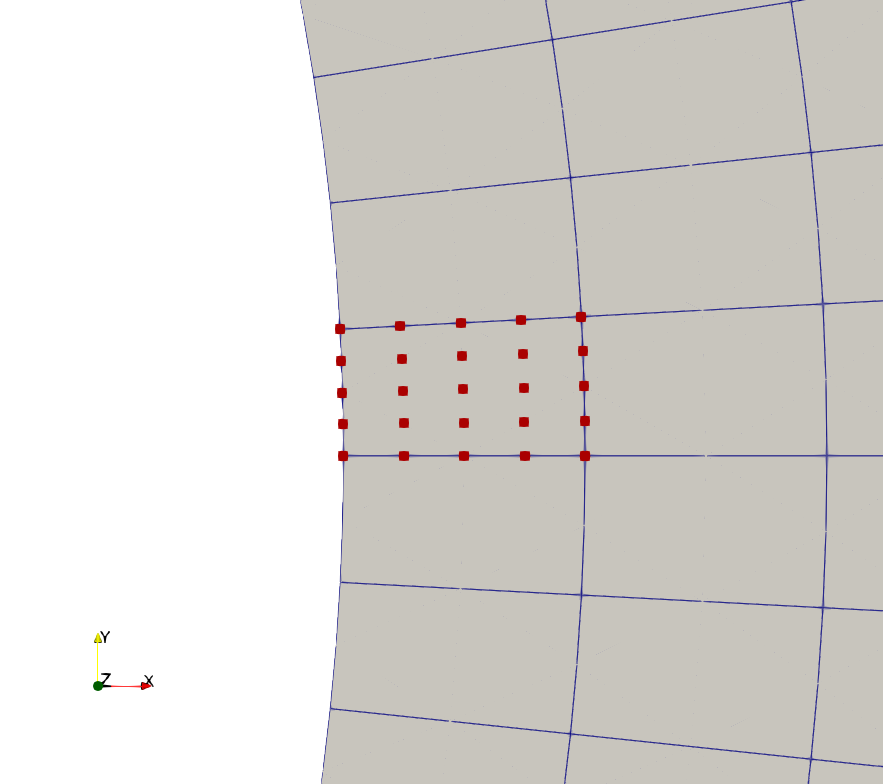
\includegraphics[width=4.2cm]{python_codes/fieldstone_152/images/mappingQ4}\\
{\captionfont Layout of the mapping nodes in element \#0 of the mesh. 
From left to right: $Q_1$, $Q_2$, $Q_3$ and $Q_4$. Rows of nodes are placed 
on concentric circles and columns of nodes are equidistant in $\theta$ space.} 
\end{center}

The code for this \stone is based on \stone~\ref{f21}.  
For each element we store the coordinates of these mapping points into two 
arrays:
\begin{lstlisting}
xmapping=np.zeros((X,nel),dtype=np.float64)
ymapping=np.zeros((X,nel),dtype=np.float64)
\end{lstlisting}
where {\python X} stands for the number of nodes for each mapping.

The reduced coordinates for the quadrature points are given by 
the Gauss-Legendre quadrature approach. The real coordinates of these points
is a function of the mapping used so that 
\begin{lstlisting}
for iel in range(0,nel):
    for kq in range(0,nqel):
        rq=qcoords_r[kq]
        sq=qcoords_s[kq]
        NNNV=NNN(rq,sq,mapping)
        xq=np.dot(NNNV[:],xmapping[:,iel])
        yq=np.dot(NNNV[:],ymapping[:,iel])
\end{lstlisting}
Likewise the Jacobian matrix is by definition a function of the chosen mapping 
so that 
\begin{lstlisting}
for iel in range(0,nel):
    for kq in range(0,nqel):
        rq=qcoords_r[kq]
        sq=qcoords_s[kq]
        dNNNVdr=dNNNdr(rq,sq,mapping)
        dNNNVds=dNNNds(rq,sq,mapping)
        jcb[0,0]=np.dot(dNNNVdr[:],xmapping[:,iel])
        jcb[0,1]=np.dot(dNNNVdr[:],ymapping[:,iel])
        jcb[1,0]=np.dot(dNNNVds[:],xmapping[:,iel])
        jcb[1,1]=np.dot(dNNNVds[:],ymapping[:,iel])
        jcob=np.linalg.det(jcb)
        jcbi=np.linalg.inv(jcb)
\end{lstlisting}


\begin{center}
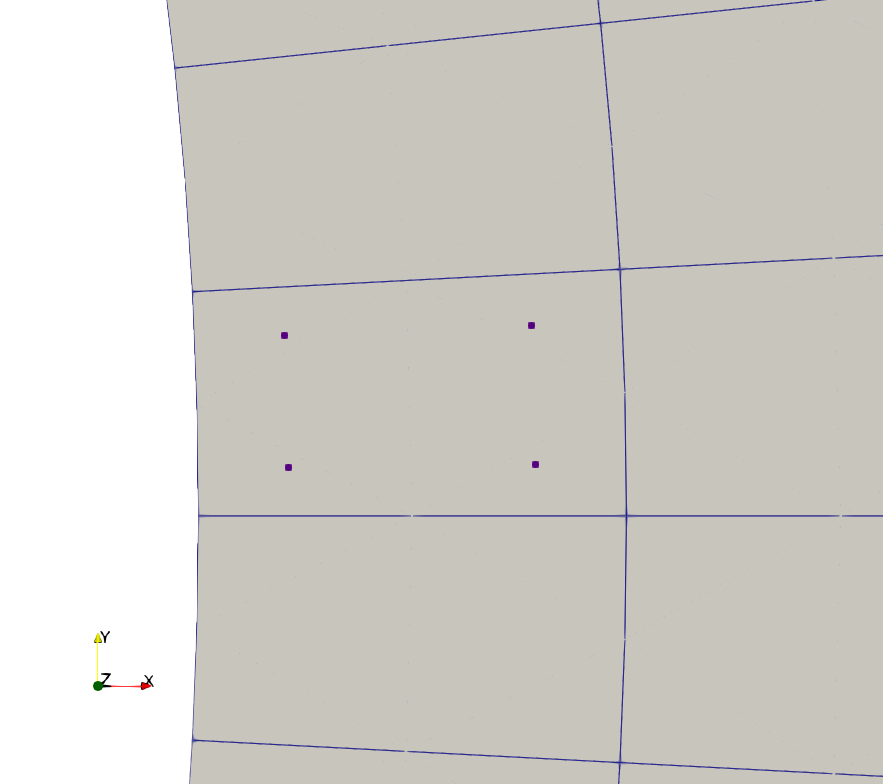
\includegraphics[width=4.2cm]{python_codes/fieldstone_152/images/nq4}
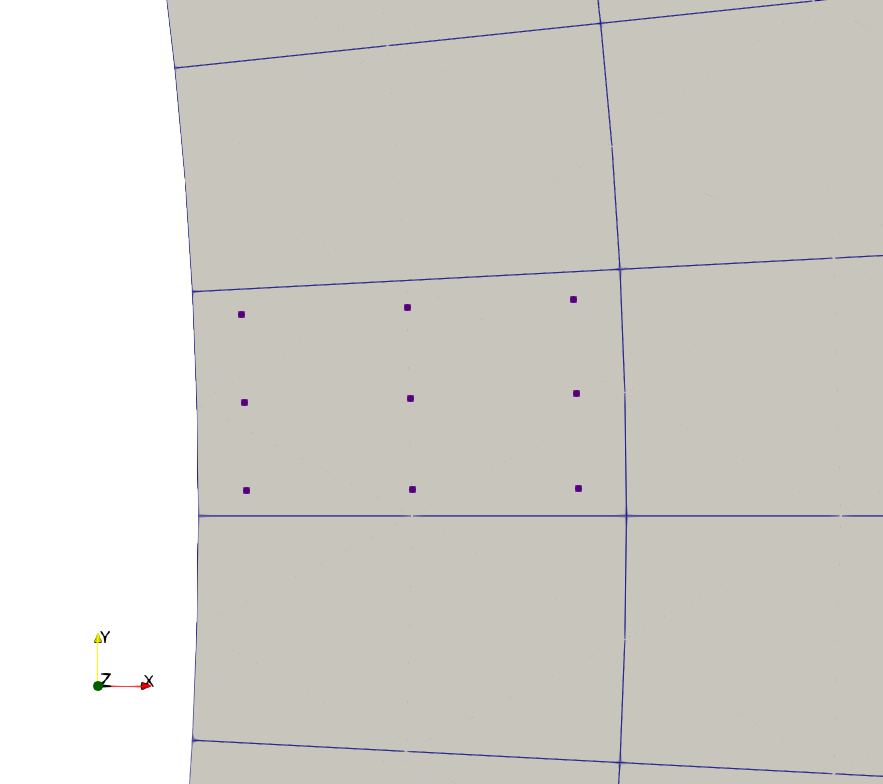
\includegraphics[width=4.2cm]{python_codes/fieldstone_152/images/nq9}
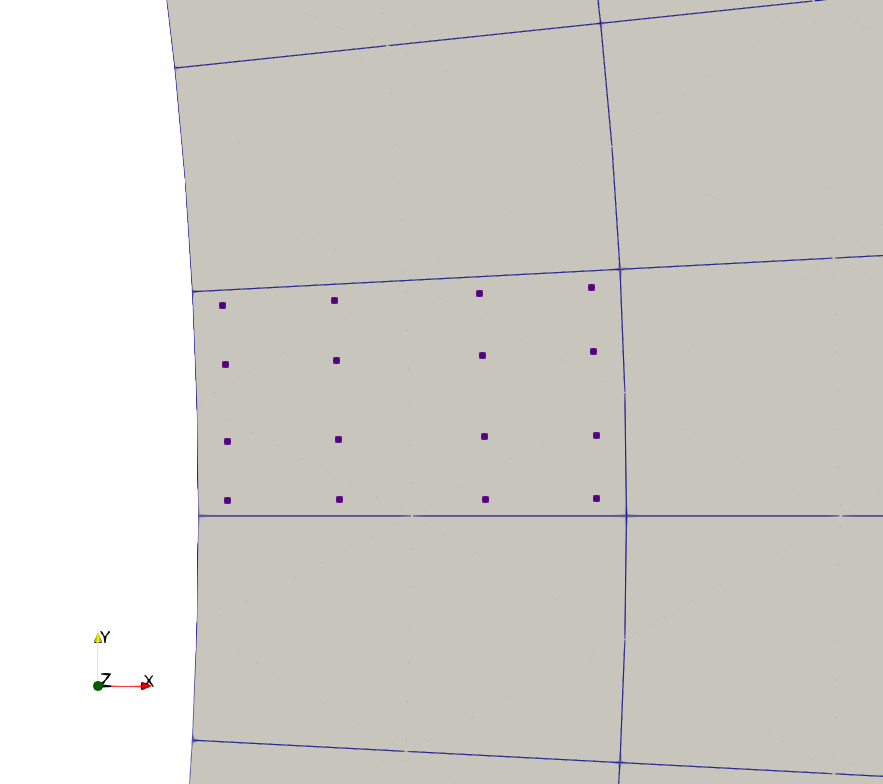
\includegraphics[width=4.2cm]{python_codes/fieldstone_152/images/nq16}
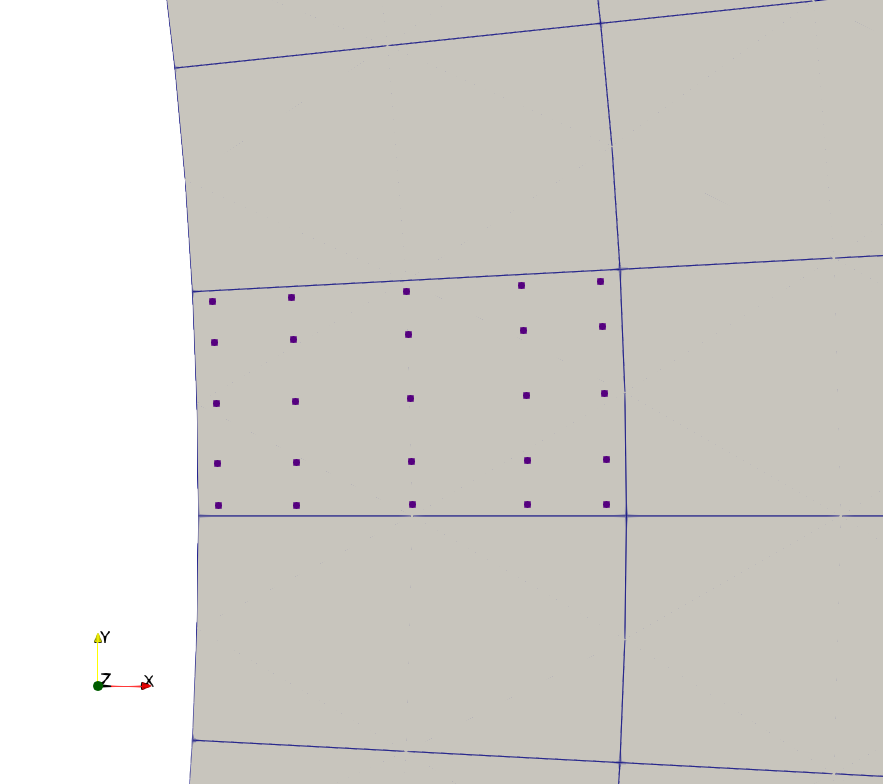
\includegraphics[width=4.2cm]{python_codes/fieldstone_152/images/nq25}\\
{\captionfont Layout of the quadrature points in element \#0 of the mesh. 
From left to right: {\python nqperdim=2,3,4,5}.} 
\end{center}

Note that the {\python axisymmetric} flag controls whether the Stokes equations 
are solved in plane strain or under the assumption that there is axisymmetry. 
In the latter case the mesh is a demi-annulus in the $x>0$ half plane.

Finally free slip boundary conditions have been implemented, but only at the 
surface, and only with the method of Lagrange Multipliers (\stone~\ref{f151}
taught us that it works as well as the other method).  


%%%%%%%%%%%%%%%%%%%%%%%%%%%%%%%%%%%%%%%
\section*{Axisymmetric considerations}

We here rely on axisymmetric cylindrical coordinates, see Section~\ref{MMM-ss:axicyleqs}.
As shown on the following figure we assume that the deformation/flow is independent of the angle 
$\theta$ so that the remaining space coordinates are $r$ and $z$.
\begin{center}
\input{tikz/tikz_axi}
\end{center}

Given the symmetry of the problem any term containing $\partial_\theta$ or $\upnu_\theta$ is zero.
The strain rate tensor given in Section~\ref{MMM-ss:srcc} then simplifies to:

\begin{eqnarray}
\dot\varepsilon_{rr} 
&=& \frac{\partial \upnu_r}{\partial r} \nn\\
\dot\varepsilon_{\theta\theta}  &=& \frac{\upnu_r}{r} \nn\\
\dot\varepsilon_{\theta r} = \dot\varepsilon_{r\theta}  &=& 0 \nn\\
\dot\varepsilon_{zz} &=& \frac{\partial \upnu_z}{\partial z} \nn\\
\dot{\varepsilon}_{rz} = \dot{\varepsilon}_{zr} 
&=& \frac{1}{2}\left( \frac{\partial \upnu_r}{\partial z} + \frac{\partial \upnu_z}{\partial r} \right) \nn\\
\dot{\varepsilon}_{\theta z} = \dot{\varepsilon}_{z \theta} &=& 0 \nn
\end{eqnarray}
Note that the term $\dot\varepsilon_{\theta\theta} $ is not zero!
The deviatoric stress tensor ${\bm \tau}=2\eta \dot{\bm \varepsilon}$ can be computed
as well as the full stress tensor ${\bm \sigma}=-p {\bm 1} + {\bm \tau}$. 


In cylindrical coordinates, and in the axisymmetric case
the strain rate tensor is given by
\[
\dot{\bm\varepsilon}(\vec\upnu)
=
\left(
\begin{array}{ccc}
\dot\varepsilon_{rr} & 0 & \dot{\varepsilon}_{rz} \\
0 & \dot{\varepsilon}_{\theta\theta}  & 0 \\
\dot{\varepsilon}_{zr} & 0 & \dot\varepsilon_{zz}
\end{array}
\right)
\]





\newpage
%%%%%%%%%%%%%%%%%%%%%%%%%%%%%%%%%%%%%%%%%%%%%%%%%%%%%%%%
\section*{Computing normals - axisymmetric case only}

As seen in \stone~\ref{f151}, there are (at least) two ways to compute the normal at the
nodes on the surface: $\vec{n}_1$ which is purely geometric and $\vec{n}_2$ which is based 
on an integration of the basis function derivatives.
We found that in the case of the annulus the two coincided to machine precision. 
Let us now turn the half annulus. As an experiment, {\it all} nodes on the hull are flagged
and the normal $\vec{n}_2$ is computed. 
Since this normal is a function of basis functions and requires an integration 
over elements, we can ask ourselves whether the mapping and/or the number
of quadrature points influence the results of the normal calculations.
The {\tt script\_normals} bash script runs the required models - note that the
$Q_1$ mapping and nqperdim=2 have been removed from the loops.

\begin{center}
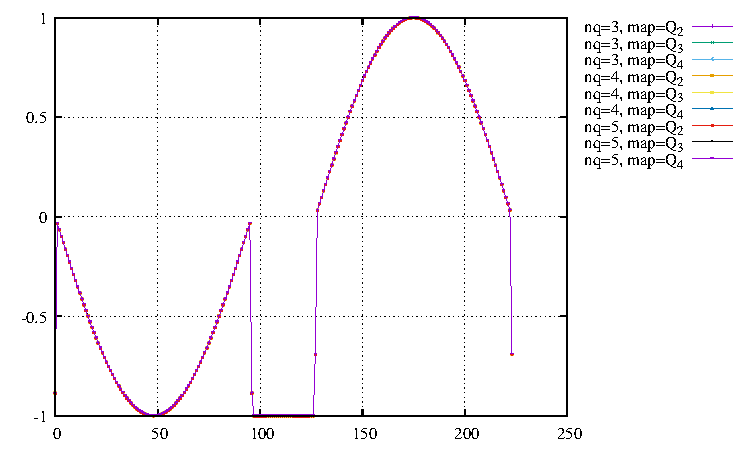
\includegraphics[width=8cm]{python_codes/fieldstone_152/results/normals/nx}
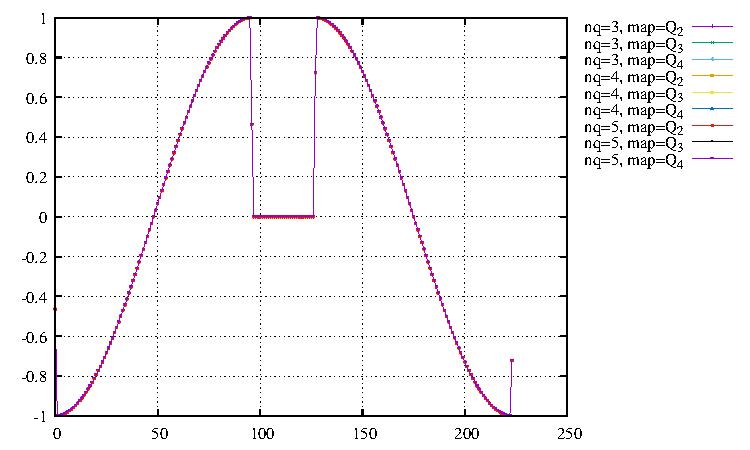
\includegraphics[width=8cm]{python_codes/fieldstone_152/results/normals/ny}\\
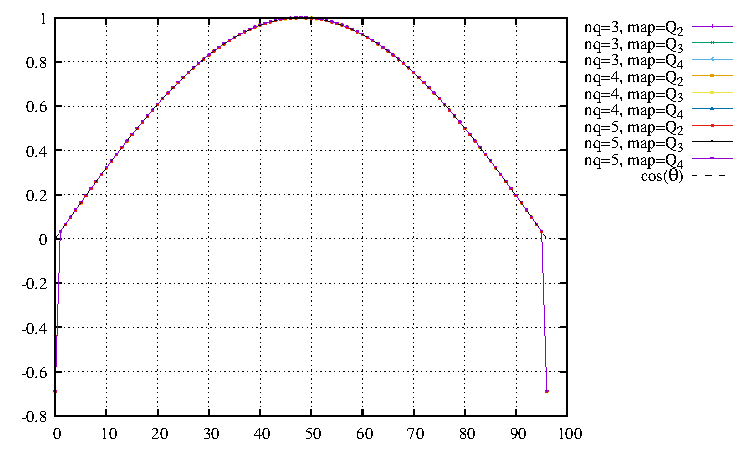
\includegraphics[width=8cm]{python_codes/fieldstone_152/results/normals/nnx}
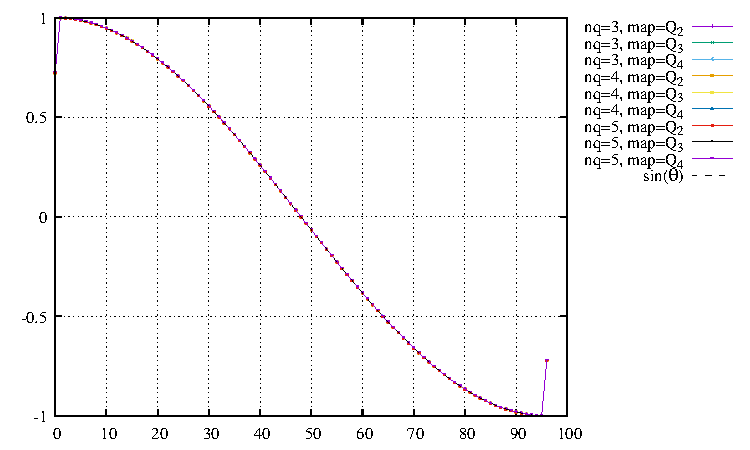
\includegraphics[width=8cm]{python_codes/fieldstone_152/results/normals/nny}\\
{\captionfont components of the normal vector on the hull (first line),
on the surface (second line). Mesh is 8x96.}
\end{center}

We find that these normal vector components do not seem to depend on the mapping nor quadrature,
and that on the curved parts they match their geometrical counterparts $\vec{n}_1$.
These normal vectors are shown here:

\begin{center}
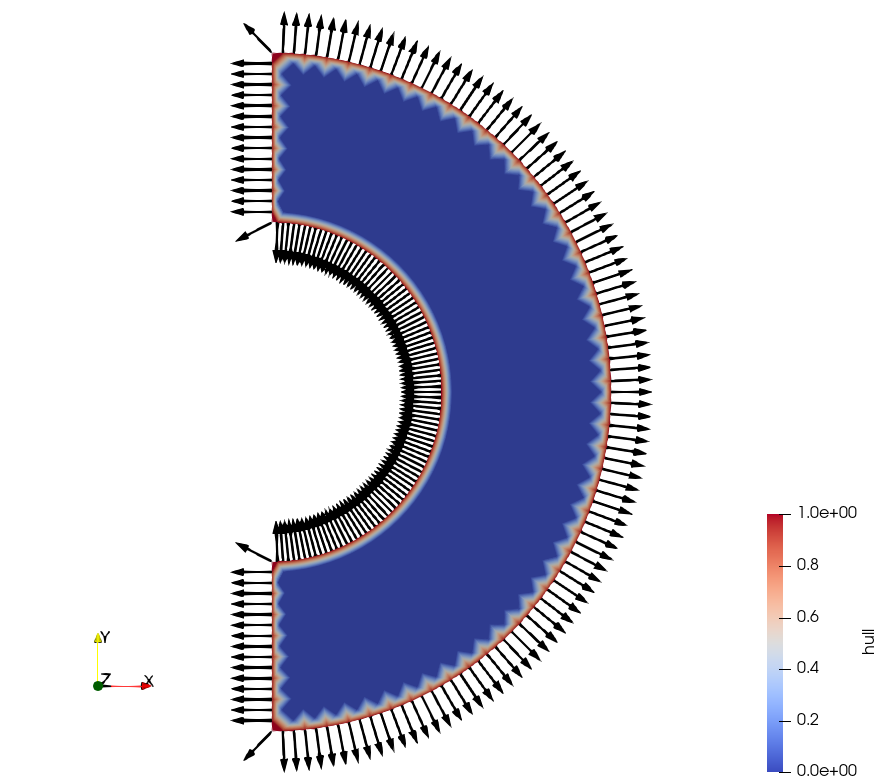
\includegraphics[width=6cm]{python_codes/fieldstone_152/results/normals/normals}
\end{center}

Obviously, we need to look closer at the four nodes that belong to the surface and the cmb with $x=0$.
On the one hand they belong the vertical boundary $x=0$ so their horizontal velocity component should be zero (axisymmetry).
On the other hand they also belong to the curved boundaries. In the case of a near infinite resolution the 
normal to the curved part would align with the vertical axis so that we would then have $v=0$. 
In the end these 4 points should be prescribed no-slip boundary conditions.

In our case here only the surface can be prescribed free slip boundary conditions and there are {\python nnt} points at the surface.
Removing the 2 extremities, we have {\python nnt-2} Lagrange multipliers. Note that then how we compute normals is not relevant.

\begin{center}
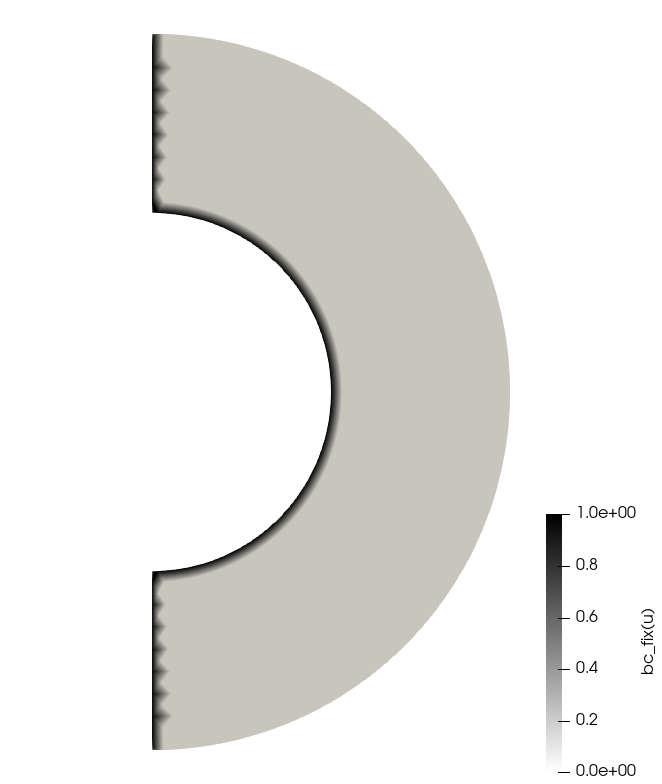
\includegraphics[width=6cm]{python_codes/fieldstone_152/images/bcfix_u}
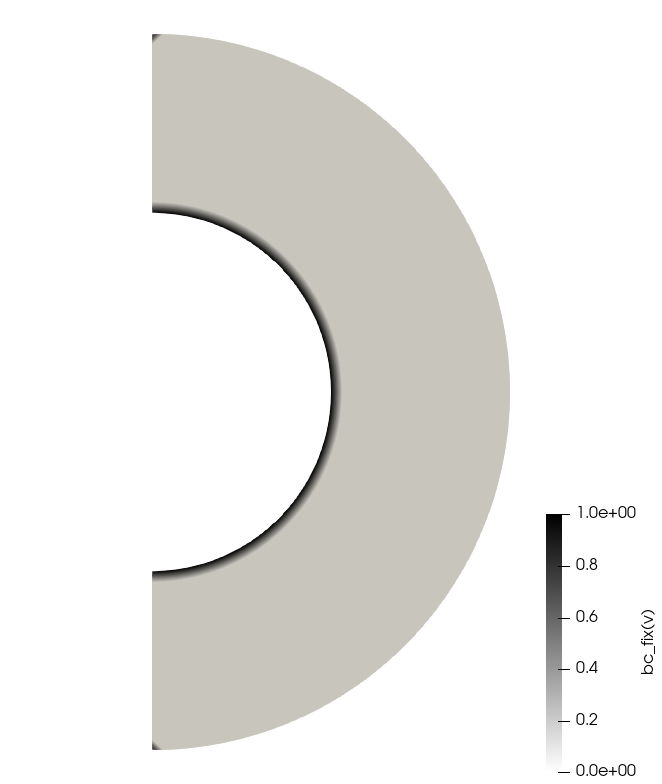
\includegraphics[width=6cm]{python_codes/fieldstone_152/images/bcfix_v}\\
{\captionfont horizontal and vertical boundary condition indicators.}
\end{center}

%%%%%%%%%%%%%%%%%%%%%%%%%%%%%%%
\section*{Pressure normalisation}

%-------------------------
\subsection*{Plane strain}

In polar coordinates the surface element is 
\[
dS = R d\theta
\]
so that 
$\int_0^{2\pi} dS = 2 \pi R$ which is the perimeter of the circle.

We wish to normalise the pressure so that it is on average zero on the surface:
\[
p_{normalised} = p - <p>
\]
where 
\[
<p> 
= \frac{\int p(r, \theta) dS }{\int dS}
= \frac{\int p(\theta) R d\theta }{\int R d \theta d\theta}
= \frac{1}{2 \pi R} R \int p(\theta) d\theta 
= \frac{1}{2 \pi }  \int_0^{2\pi} p(\theta) d\theta 
\]


%------------------------------
\subsection*{Axisymmetric case}

\begin{center}
\includegraphics[width=2cm]{images/sphcoord}
\end{center}

In spherical coordinates, the surface element is 
\[
dS= R^2 \sin \theta d\theta d\phi
\]
We wish to normalise the pressure so that it is on average zero on the surface:
\[
p_{normalised} = p - <p>
\]
where 
\[
<p> 
= \frac{\iint p(\theta,\phi) dS }{\iint dS}
= \frac{\iint p(\theta,\phi) R^2 \sin \theta d\theta d\phi}{\iint R^2 \sin \theta d\theta d\phi}
\]
and since $p$ is independent of $\phi$ then 
\[
<p> 
= \frac{R_2^2 \cdot 2\pi \cdot  \int_0^\pi p(\theta)  \sin \theta d\theta}
{R_2^2 \cdot 2\pi \cdot \int  \sin \theta d\theta }
= \frac{ 2\pi R_2^2 \int_0^\pi p(\theta)  \sin \theta d\theta} {4\pi R_2^2}
\]
The integral over $\theta$ can be simplified by using the average pressure 
along the edge and the angle of the edge middle point:
\begin{lstlisting}
poffset=0
for iel in range(0,nel):
    if surface_element[iel]:
       dtheta=theta_sph[iconV[2,iel]]-theta_sph[iconV[3,iel]]
       pmean=0.5*(p[iconP[2,iel]]+p[iconP[3,iel]])
       poffset+=np.sin((theta_sph[iconV[2,iel]]+theta_sph[iconV[3,iel]])/2)*dtheta\
                *2*np.pi*R2**2 * pmean
poffset/=4*np.pi*R2**2
\end{lstlisting}



%%%%%%%%%%%%%%%%%%%%%%%%%%%%%%%
\section*{On the use of ASPECT}

I have produced two input files for \aspect that carry out experiment 2.
One is 2D (plane strain), the other one is 3D. 
Input files and their results are included in the corresponding results folder.


%%%%%%%%%%%%%%%%%%%%%%%%%%%%%%%%%%%%%%%%%%%%%%%%%%%%%%%%%%%%%
\section*{From Cartesian to Spherical coordinates}

In order to compute the dynamic topography we will need $\sigma_{rr}$, 
which in fact will require $\dot{\varepsilon}_{rr}$. This means that 
having obtained the strain rate tensor in Cartesian coordinates we must 
rewrite it in spherical coordinates with the following conventions:

\begin{center}
\includegraphics[width=3cm]{images/sphcoord}
\end{center}

We have
\begin{eqnarray}
{\bm T}_{\tiny Sph}&=&
\left(
\begin{array}{ccc}
T_{rr}       & T_{r\theta}      & T_{r\phi} \\
T_{\theta r} & T_{\theta\theta} & T_{\theta\phi} \\
T_{\phi r}   & T_{\phi \theta}  & T_{\phi\phi}
\end{array}
\right) \nn\\
&=&
\left(
\begin{array}{ccc}
\sin\theta \cos\phi & \sin\theta \sin\phi & \cos\theta \\
\cos\theta \cos\phi & \cos\theta \sin\phi & -\sin\theta \\
-\sin\phi & \cos\phi & 0 
\end{array}
\right)
\cdot
\left(
\begin{array}{ccc}
T_{xx} & T_{xy} & T_{xz} \\
T_{yx} & T_{yy} & T_{yz} \\
T_{zx} & T_{zy} & T_{zz} 
\end{array}
\right)
\cdot
\left(
\begin{array}{ccc}
\sin\theta\cos\phi & \cos\theta\cos\phi & -\sin\phi \\
\sin\theta\sin\phi & \cos\theta\sin\phi & \cos\phi \\
\cos\theta & -\sin\theta & 0
\end{array}
\right) 
\nn\\
{\bm T}_{\tiny Cart} &=&
\left(
\begin{array}{ccc}
T_{xx} & T_{xy} & T_{xz} \\
T_{yx} & T_{yy} & T_{yz} \\
T_{zx} & T_{zy} & T_{zz} 
\end{array}
\right) \nn\\
&=&
\left(
\begin{array}{ccc}
\sin\theta\cos\phi & \cos\theta\cos\phi & -\sin\phi \\
\sin\theta\sin\phi & \cos\theta\sin\phi & \cos\phi \\
\cos\theta & -\sin\theta & 0
\end{array}
\right)
\cdot
\left(
\begin{array}{ccc}
T_{rr}       & T_{r\theta}      & T_{r\phi} \\
T_{\theta r} & T_{\theta\theta} & T_{\theta\phi} \\
T_{\phi r}   & T_{\phi \theta}  & T_{\phi\phi}
\end{array}
\right)
\cdot
\left(
\begin{array}{ccc}
\sin\theta \cos\phi & \sin\theta \sin\phi & \cos\theta \\
\cos\theta \cos\phi & \cos\theta \sin\phi & -\sin\theta \\
-\sin\phi & \cos\phi & 0 
\end{array}
\right) \nonumber
\end{eqnarray}
In our case, calculations take place in the 
$(x,z)$-plane so we have $\phi=0$ and the equation above 
becomes
\[
\left(
\begin{array}{ccc}
T_{rr}       & T_{r\theta}      & T_{r\phi} \\
T_{\theta r} & T_{\theta\theta} & T_{\theta\phi} \\
T_{\phi r}   & T_{\phi \theta}  & T_{\phi\phi}
\end{array}
\right)
=
\left(
\begin{array}{ccc}
\sin\theta  & 0 & \cos\theta \\
\cos\theta  & 0 & -\sin\theta \\
0 & 1 & 0 
\end{array}
\right)
\cdot
\left(
\begin{array}{ccc}
T_{xx} & T_{xy} & T_{xz} \\
T_{yx} & T_{yy} & T_{yz} \\
T_{zx} & T_{zy} & T_{zz} 
\end{array}
\right)
\cdot
\left(
\begin{array}{ccc}
\sin\theta & \cos\theta & 0 \\
0 & 0 & 1 \\
\cos\theta & -\sin\theta & 0
\end{array}
\right)
\]
We define $c_\theta=\cos\theta$, $s_\theta=\sin\theta$ so that
\[
\left(
\begin{array}{ccc}
T_{rr}       & T_{r\theta}      & T_{r\phi} \\
T_{\theta r} & T_{\theta\theta} & T_{\theta\phi} \\
T_{\phi r}   & T_{\phi \theta}  & T_{\phi\phi}
\end{array}
\right)
=
\left(
\begin{array}{ccc}
s_\theta  & 0 & c_\theta \\
c_\theta  & 0 & -s_\theta \\
0 & 1 & 0 
\end{array}
\right)
\cdot
\left(
\begin{array}{ccc}
T_{xx} & T_{xy} & T_{xz} \\
T_{yx} & T_{yy} & T_{yz} \\
T_{zx} & T_{zy} & T_{zz} 
\end{array}
\right)
\cdot
\left(
\begin{array}{ccc}
s_\theta & c_\theta & 0 \\
0 & 0 & 1 \\
c_\theta & -s_\theta & 0
\end{array}
\right)
\]
As we have seen above we have 
\[
\dot{\bm\varepsilon}_{\tiny Cart}
=
\left(
\begin{array}{ccc}
\dot\varepsilon_{xx} & 0 & \dot{\varepsilon}_{xz} \\
0 & \dot{\varepsilon}_{yy}  & 0 \\
\dot{\varepsilon}_{xz} & 0 & \dot\varepsilon_{zz}
\end{array}
\right)
\]
so 
\begin{eqnarray}
\dot{\bm \varepsilon}_{\tiny Sph}=
\left(
\begin{array}{ccc}
\dot\varepsilon_{rr}       & \dot\varepsilon_{r\theta}      & \dot\varepsilon_{r\phi} \\
\dot\varepsilon_{\theta r} & \dot\varepsilon_{\theta\theta} & \dot\varepsilon_{\theta\phi} \\
\dot\varepsilon_{\phi r}   & \dot\varepsilon_{\phi \theta}  & \dot\varepsilon_{\phi\phi}
\end{array}
\right)
&=&
\left(
\begin{array}{ccc}
s_\theta  & 0 & c_\theta \\
c_\theta  & 0 & -s_\theta \\
0 & 1 & 0 
\end{array}
\right)
\cdot
\left(
\begin{array}{ccc}
\dot\varepsilon_{xx} & 0 & \dot{\varepsilon}_{xz} \\
0 & \dot{\varepsilon}_{yy}  & 0 \\
\dot{\varepsilon}_{xz} & 0 & \dot\varepsilon_{zz}
\end{array}
\right)
\cdot
\left(
\begin{array}{ccc}
s_\theta & c_\theta & 0 \\
0 & 0 & 1 \\
c_\theta & -s_\theta & 0
\end{array}
\right)  \nonumber\\
&=&
\left(
\begin{array}{ccc}
s_\theta  & 0 & c_\theta \\
c_\theta  & 0 & -s_\theta \\
0 & 1 & 0 
\end{array}
\right)
\cdot
\left(
\begin{array}{ccc}
\dot\varepsilon_{xx} s_\theta + 
\dot\varepsilon_{xz} c_\theta  & 
\dot\varepsilon_{xx} c_\theta - 
\dot\varepsilon_{xz} s_\theta  &
0 \\
0 & 0 & \dot{\varepsilon}_{yy}  
\\
\dot\varepsilon_{xz} s_\theta + 
\dot\varepsilon_{zz} c_\theta  &
\dot\varepsilon_{xz} c_\theta - 
\dot\varepsilon_{zz} s_\theta  &
0 
\end{array}
\right)  \nonumber\\
&=&
\left(
\begin{array}{ccc}
\dot\varepsilon_{xx} s_\theta^2 + 
2 \dot\varepsilon_{xz} c_\theta  s_\theta +
\dot\varepsilon_{zz} c_\theta ^2  
& 
\dot\varepsilon_{xx} c_\theta s_\theta - 
\dot\varepsilon_{xz} s_\theta^2  +
\dot\varepsilon_{xz} c_\theta^2 - 
\dot\varepsilon_{zz} s_\theta c_\theta 
& 0 \\ \\
\dot\varepsilon_{xx} s_\theta c_\theta+ 
\dot\varepsilon_{xz} c_\theta^2  -
\dot\varepsilon_{xz} s_\theta^2 -
\dot\varepsilon_{zz} c_\theta s_\theta 
&
\dot\varepsilon_{xx} c_\theta^2 - 
2\dot\varepsilon_{xz} s_\theta c_\theta +
\dot\varepsilon_{zz} s_\theta^2  
& 0 
\\ \\
0 & 0 & \dot{\varepsilon}_{yy} 
\end{array}
\right)  \nonumber
\end{eqnarray}
We can easily verify that the trace of this tensor is zero.

In the code we need to be careful and use {\python theta\_sph}:

\begin{center}
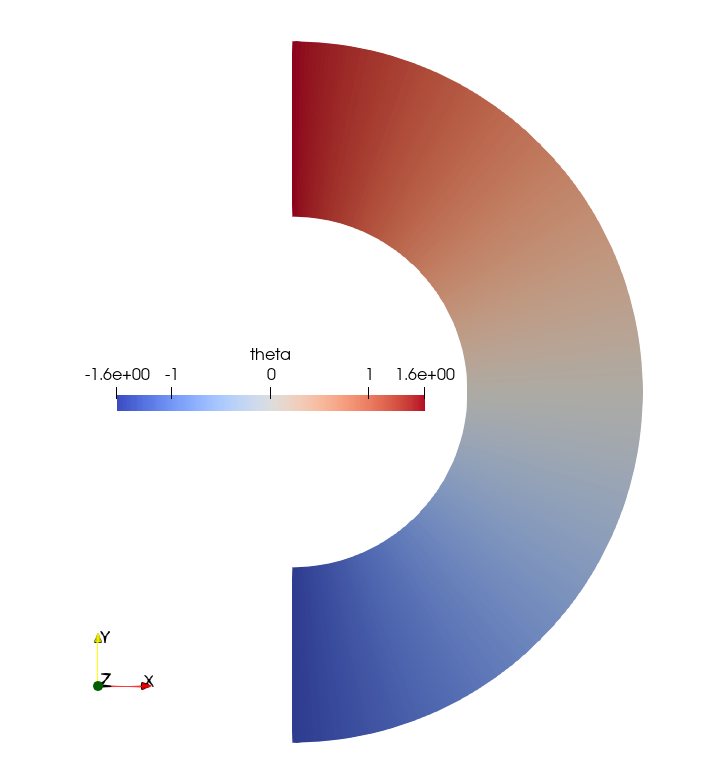
\includegraphics[width=8.3cm]{python_codes/fieldstone_152/images/theta}
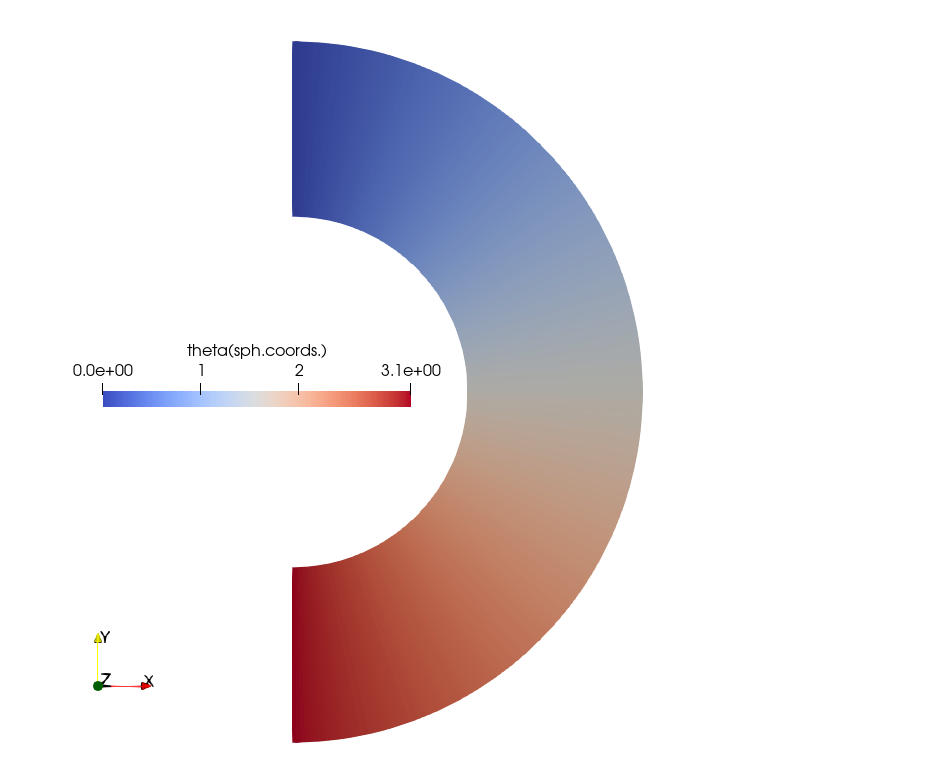
\includegraphics[width=8.3cm]{python_codes/fieldstone_152/images/theta_sph}
\end{center}

\begin{lstlisting}
for i in range(0,NV):
    theta_sph[i]=np.pi/2-math.atan(yV[i]/abs(xV[i]))
    if xV[i]>=0:
       e_rr[i]=exx2[i]*np.sin(theta_sph[i])**2+\
               2*exy2[i]*np.sin(theta_sph[i])*np.cos(theta_sph[i])+\
               eyy2[i]*np.cos(theta_sph[i])**2
       e_tt[i]=exx2[i]*np.cos(theta_sph[i])**2-\
               2*exy2[i]*np.sin(theta_sph[i])*np.cos(theta_sph[i])+\
               eyy2[i]*np.sin(theta_sph[i])**2
       e_rt[i]=(exx2[i]-eyy2[i])*np.sin(theta_sph[i])*np.cos(theta_sph[i])+\
               exy2[i]*(-np.sin(theta_sph[i])**2+\
               np.cos(theta_sph[i])**2)
\end{lstlisting}




%%%%%%%%%%%%%%%%%%%%%%%%%%%%%%%
\section*{Dynamic topography}

Looking at the \aspect manual, we find:

``we evaluate the stress and evaluate the component of it in the direction in which 
gravity acts. In other words we compute 
\[
\sigma_{rr}={\hat g}^T (2 \eta \varepsilon(\mathbf u)
- \frac 13 (\textrm{div}\;\mathbf u)I)\hat g - p_d
\] 
where 
$\hat g = \mathbf g/\|\mathbf g\|$ is the direction of 
the gravity vector $\mathbf g$ and $p_d=p-p_a$ is the dynamic 
pressure computed by subtracting the adiabatic pressure $p_a$ 
from the total pressure $p$ computed as part of the Stokes 
solve. From this, the dynamic 
topography is computed using the formula 
\[
h=\frac{\sigma_{rr}}{(\mathbf g \cdot \mathbf n)  \rho}
\] 
where $\rho$ is the density. For the bottom surface we chose the convection 
that positive values are up (out) and negative values are in (down), analogous to 
the deformation of the upper surface. 
The file format then consists of lines with Euclidean coordinates 
followed by the corresponding topography value.''

In this \stone the viscosity is constant in the domain, the flow 
is incompressible and $\vec{g}= -g_0 \vec{e}_r$ so we can compute the 
dynamic topography as follows:
\[
h = - \frac{-p + 2 \eta_0 \dot{\varepsilon}_{rr} }{\rho_0 g_0}
\]
This is of course valid if what is above the surface is a fluid with zero density.
This translates into:

\begin{lstlisting}
dyn_topo=np.zeros(NV,dtype=np.float64)
for i in range(0,NV):
    if surfaceV[i] and xV[i]>=0:
       dyn_topo[i]= -(2*viscosity*e_rr[i]-q[i])/(rho0*g0) 
\end{lstlisting}

Note that in our case $\rho_0=1$ and $g_0=1$ so that in fact the dynamic topography 
is simply $-\sigma_{rr}$.










\newpage
%%%%%%%%%%%%%%%%%%%%%%%%%%%%%%%
\section*{Areas and volumes}

Here we simply compute 
\[
{\cal A} = \sum_e \int_{\Omega_e} d\Omega
\]
where the sum runs over all elements of the annulus
and 
\[
{\cal V} = \sum_e \int_{\Omega_e} 2\pi x d\Omega
\]
for elements on the $x>0$ side of the annulus (axisymmetric formulation)\footnote{the number of elements in the 
tangential direction is a multiple of 4, so element sides always coincide with the $y$-axis.}.
We of course have 
\[
{\cal A}_{analytical} = \pi (R_2^2-R_1^2)
\qquad\qquad
{\cal V}_{analytical} = \frac43 \pi (R_2^3-R_1^3)
\]
so that we can compute the relative errors as a function of resolution, mapping and quadrature: 
\begin{center}
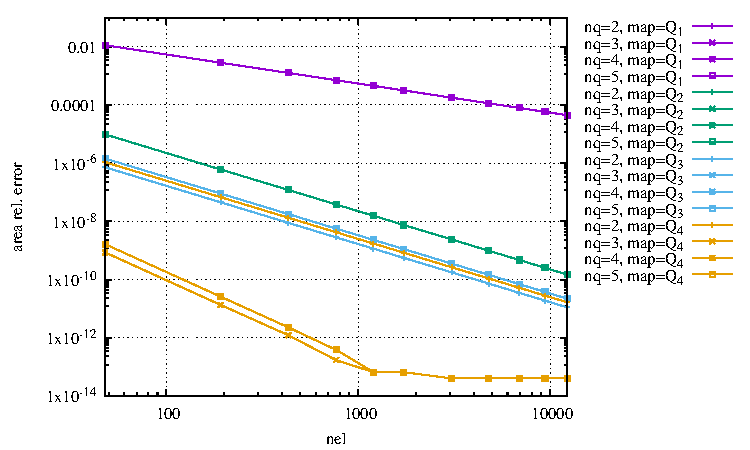
\includegraphics[width=8.3cm]{python_codes/fieldstone_152/results/areas/areas.pdf}
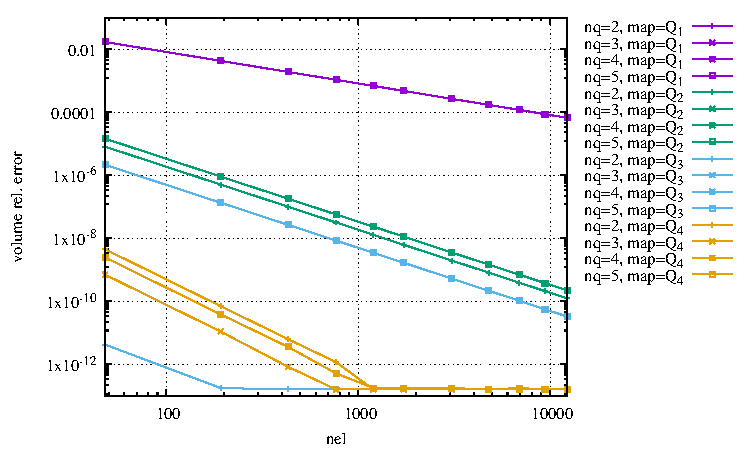
\includegraphics[width=8.3cm]{python_codes/fieldstone_152/results/areas/volumes.pdf}
\end{center}

\noindent Conclusions:
\begin{itemize}
\item unsurprisingly $Q_1$ mapping yields the worst results
\item mapping is the controling factor, much more than quadrature
\item for the isoparametric element (mapping $Q_2$) the number of quadrature points 
is not critical. Results are virtually identical for {\python nqperdim=2,3,4,5}
\item $Q_3$ about one order of magnitude more accurate than $Q_2$ 
\item $Q_4$ mapping 3-4 orders of magnitude more accurate than $Q_2$ mapping
\item I can't explain the {\python nqperdim=2 + mapping=Q3} results that outperform everything else... (volume only)
\end{itemize}

Do these results translate to the solution of the Stokes system? Let's investigate...
The provided {\tt script\_errors} bash script implements a triple loop 
over resolution, number of quadrature points and mapping type.
Results are shown in the following.

\newpage
%%%%%%%%%%%%%%%%%%%%%%%%%%%%%%%%%%%%%%%%%%%%%%%%%%%%%%%%%%%%%%%%%%%%%%%%%%%%%%%%%%%%%
\section*{Annulus convection benchmark (exp=0)}


This benchmark is documented in Section~\ref{MMM-ss:anconv}.

For reference, in this benchmark we solve the Stokes equation for an incompressible
isothermal fluid in an annulus of inner radius $R_1$
and outer radius $R_2$ with the following boundary conditions:
\begin{itemize}
\item Inner boundary: $\upnu_r(R_1,\theta)=0$ 
\item Outer boundary: $\upnu_r(R_2,\theta)=0$ 
\end{itemize}
and the manufactured solution takes the form:
\begin{eqnarray}
\upnu_\theta(r,\theta) &=& f(r) \cos(k\theta) \\
\upnu_r(r,\theta) &=& g(r) k  \sin(k\theta)  \\
p(r,\theta) &=& k h(r) \sin(k \theta) + \rho_0 g_r (r-R_2)  \\
\rho(r,\theta) &=& k \sin (k \theta) \aleph(r) + \rho_0 \\
\end{eqnarray}
with
\begin{eqnarray}
A &=& \frac{2(\ln R_1 - \ln R_2)} { R_2^2 \ln R_1  - R_1^2 \ln R_2}    \nn\\
B &=& \frac{R_2^2-R_1^2}{R_2^2 \ln R_1 - R_1^2 \ln R_2} \nn\\
f(r)   &=& Ar +\frac{B}{r} \nn\\
f'(r)  &=& A - \frac{B}{r^2} \nn\\
g(r)   &=& \frac{A}{2}r  +  \frac{B}{r} \ln r - \frac{1}{r} \nn\\
g'(r)  &=& \frac{A}{2}  +  \frac{B}{r^2} (1-\ln r)   + \frac{1}{r^2} \nn\\
g''(r) &=&  - \frac{B}{r^3} (3 - 2 \ln r )  \nn\\
h(r)   &=& \frac{1}{r^2}(2g-f) \nn\\
\aleph(r) &=&  -g'' - \frac{g'}{r} ( 1 - \frac{2}{r}) + \frac{g}{r^2} (k^2 + 1 -\frac{4}{r})  - \frac{2f}{r^2}  (1-\frac{1}{r}) - \frac{f'}{r^2}   \nn
\end{eqnarray}


\begin{center}
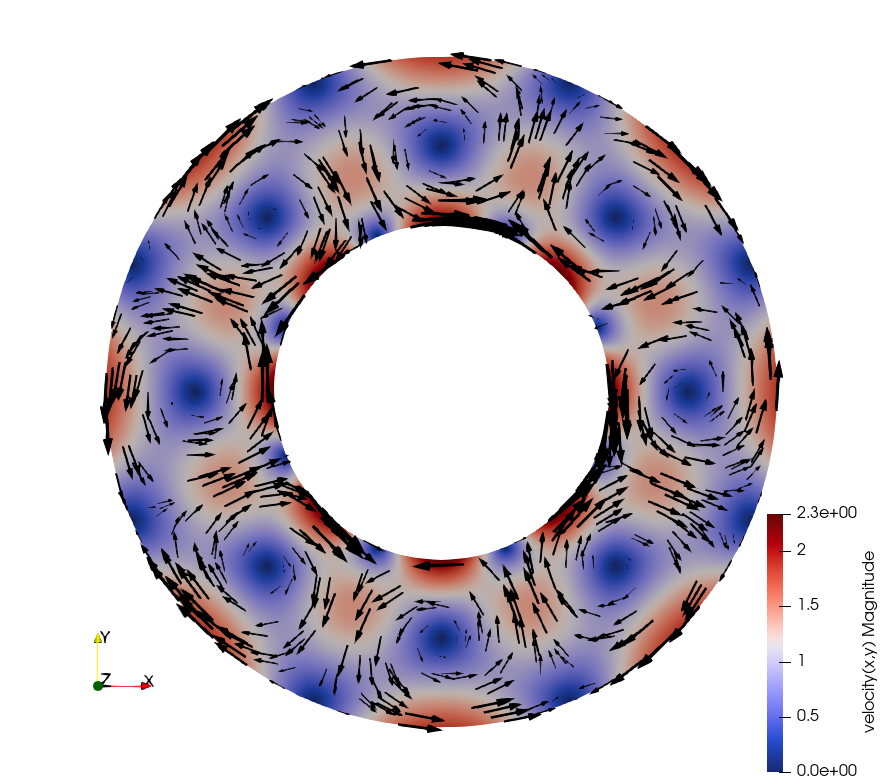
\includegraphics[width=6cm]{python_codes/fieldstone_152/images/vel}
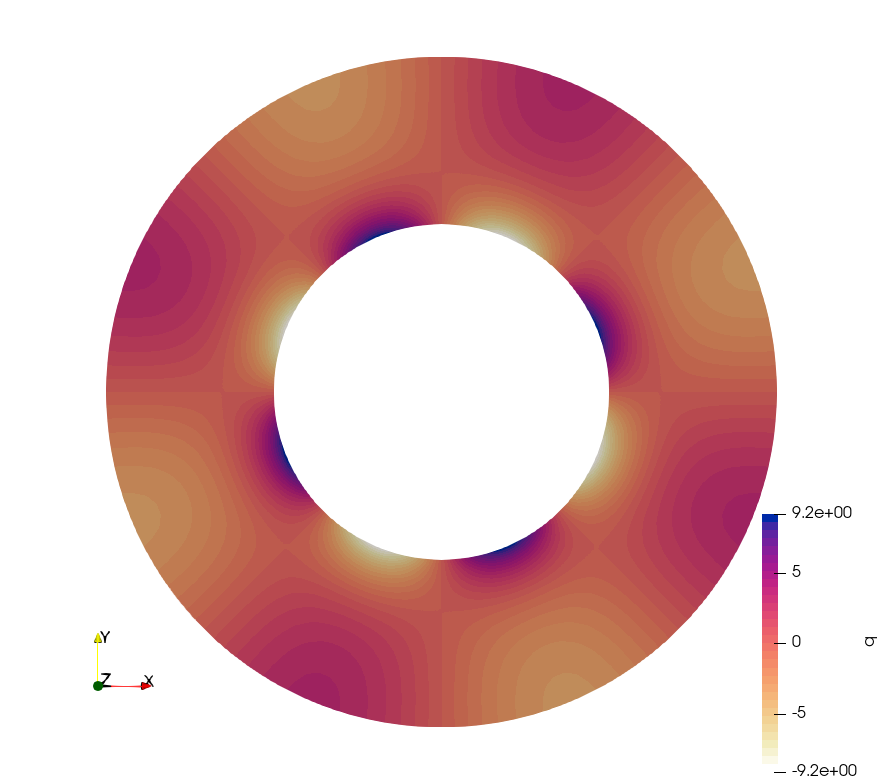
\includegraphics[width=6cm]{python_codes/fieldstone_152/images/press}\\
{\captionfont Velocity and pressure fields for $k=4$.}
\end{center}





%---------------------------------------
\subsection*{Root mean square velocity}

\begin{center}
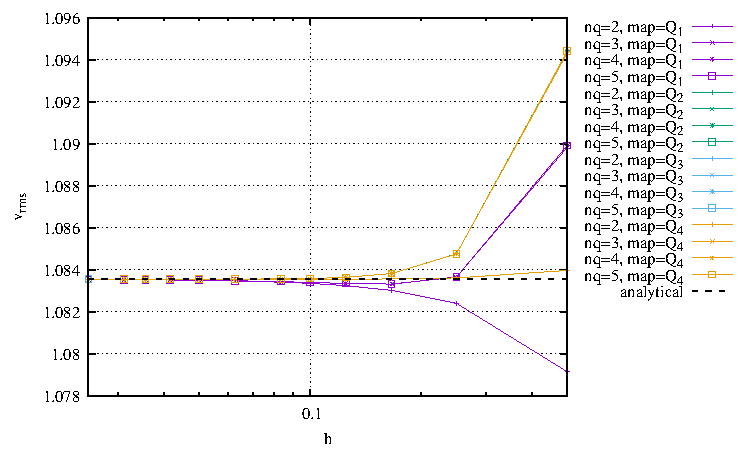
\includegraphics[width=8.3cm]{python_codes/fieldstone_152/results/exp0/vrms}
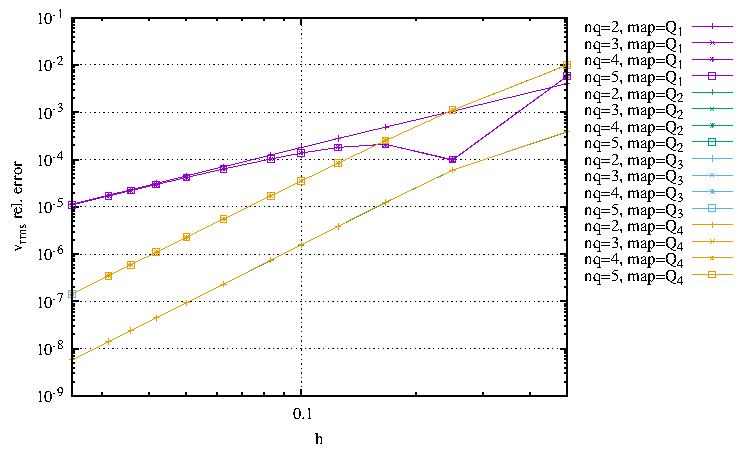
\includegraphics[width=8.3cm]{python_codes/fieldstone_152/results/exp0/vrms_error}\\
{\captionfont Note that we define $h=(R_2-R_1)/nelr=1/nelr$.}
\end{center}

As expected linear mapping yields the worst results. However results are virtually identical for 
the three other mappings.
What is very surprising is the much higher accuracy of {\python nqperdim=2} (i.e. subparametric mapping) ?!


%---------------------------------------
\subsection*{Velocity and pressure errors}

We first look at the min/max values of the nodal velocity and pressure errors over all the nodes:
\begin{center}
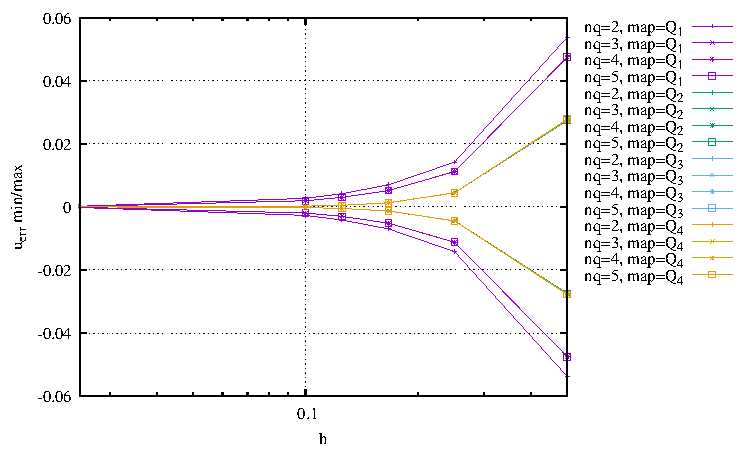
\includegraphics[width=8.3cm]{python_codes/fieldstone_152/results/exp0/u_err}
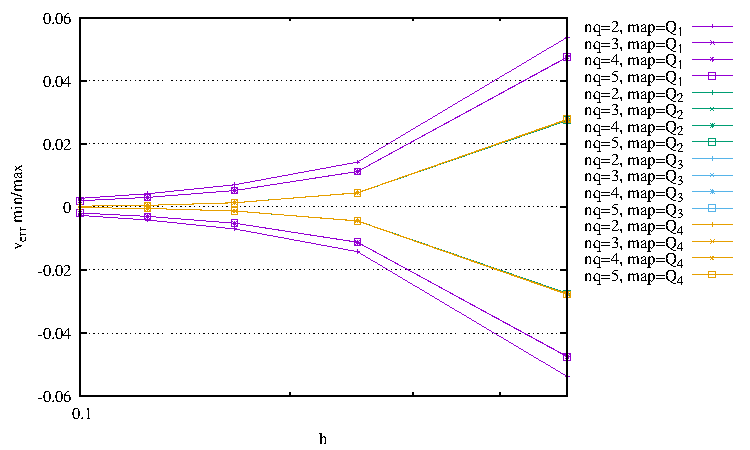
\includegraphics[width=8.3cm]{python_codes/fieldstone_152/results/exp0/v_err}\\
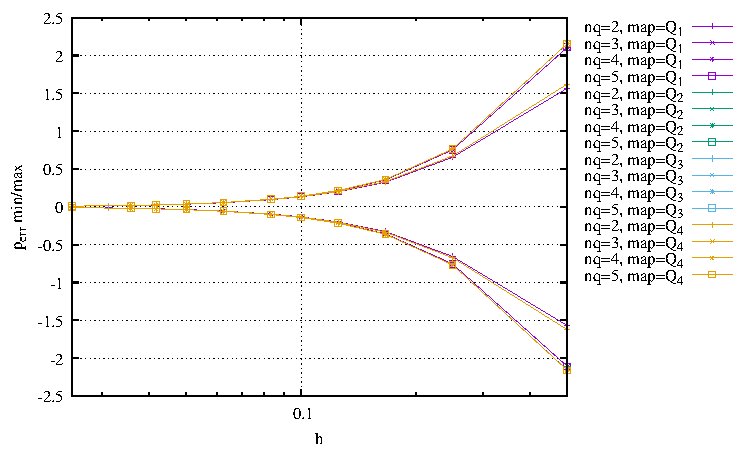
\includegraphics[width=8.3cm]{python_codes/fieldstone_152/results/exp0/p_err}
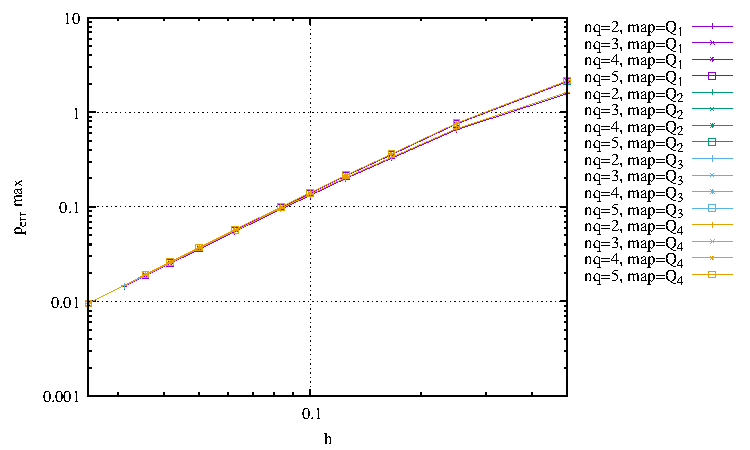
\includegraphics[width=8.3cm]{python_codes/fieldstone_152/results/exp0/p_err_max}\\
{\captionfont Top row: min/max of $u^h(x,y)-u^{th}(x,y)$ and $v^h(x,y)-v^{th}(x,y)$;
Bottom row left: min/max of $p^h(x,y)-p^{th}(x,y)$; bottom row right max of  $p^h(x,y)-p^{th}(x,y)$.} 
\end{center}
We see that all measurements decrease (in amplitude) when the resolution is increased and that 
the $Q_1$ mapping yields the largest errors. 
Interestingly the subparametric case {\python nqperdim=2} seems to yield more accurate 
pressure results.

Turning now to velocity and pressure errors in the $L_2$ norm, 
as expected with the \QtwoQone element (and already shown in \stone~\ref{f21})
we recover a cubic convergence for the velocity error and quadratic for the 
pressure... almost always.

\begin{center}
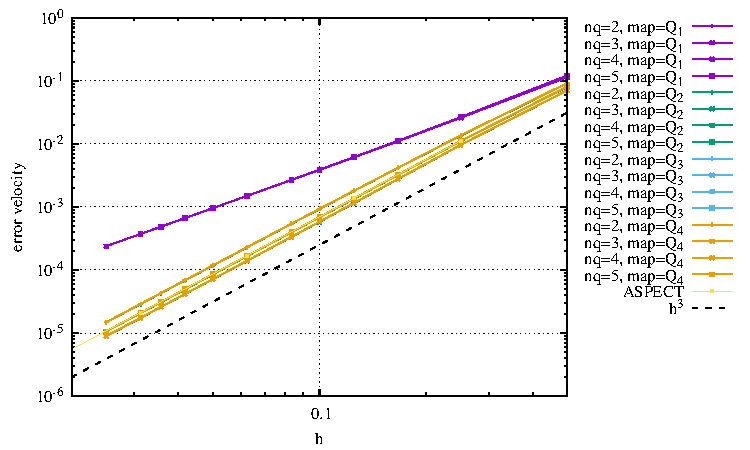
\includegraphics[width=8.3cm]{python_codes/fieldstone_152/results/exp0/errv}
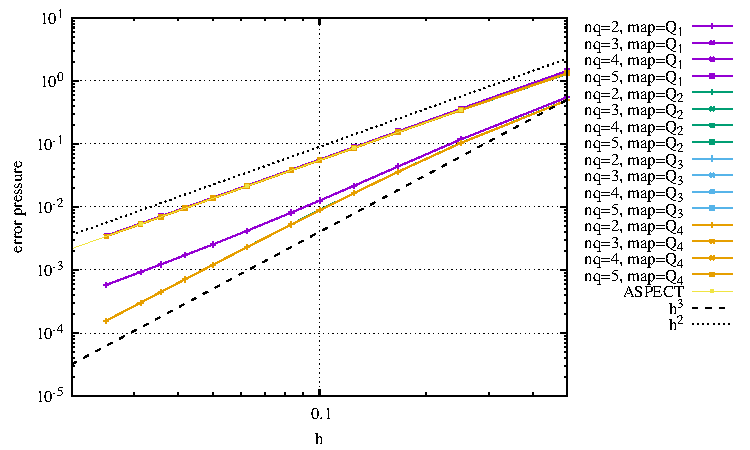
\includegraphics[width=8.3cm]{python_codes/fieldstone_152/results/exp0/errp}
\end{center}

Our velocity and pressure error measurements are identical to those of \aspect.
But why does the subparametric mapping yield a pressure error that is superconvergent?

%IDEA/THOUGHT: are these q points superconvergent points? find ref!

\newpage

%---------------------------------------
\subsection*{Strain rate errors}

Since the analytical velocity field is known so are the strain rate tensor components.
Similarly to \stone~21 this code computes the nodal strain rate components
in three different ways. 
\begin{itemize}
\item method \#1: strain rate components are computed in the middle of the element and then averaged over elements sharing a node.
\item method \#2: strain rate components are computed at each node of the element and then averaged over elements sharing a node.
\item method \#3: global recovery process as documented in Section~\ref{MMM-ss:gradrecovery}.
\end{itemize}

Errors are then computed in the same way as the velocity components.

\begin{center}
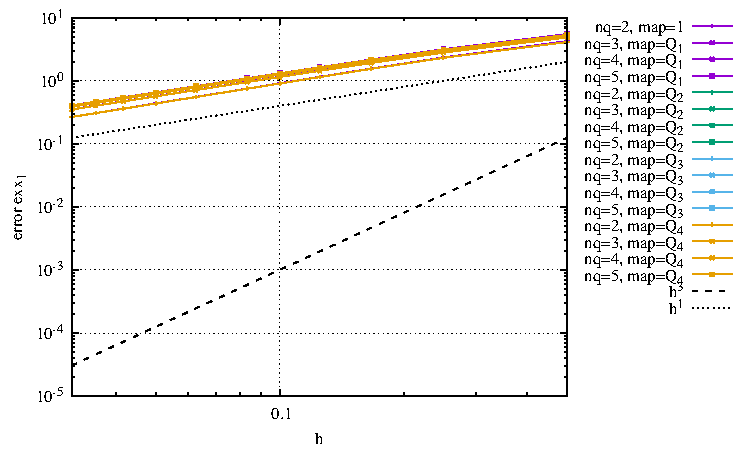
\includegraphics[width=5.7cm]{python_codes/fieldstone_152/results/exp0/err_exx1}
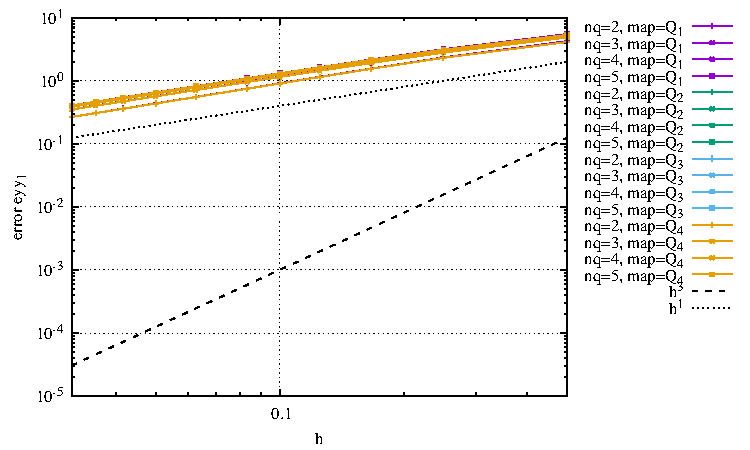
\includegraphics[width=5.7cm]{python_codes/fieldstone_152/results/exp0/err_eyy1}
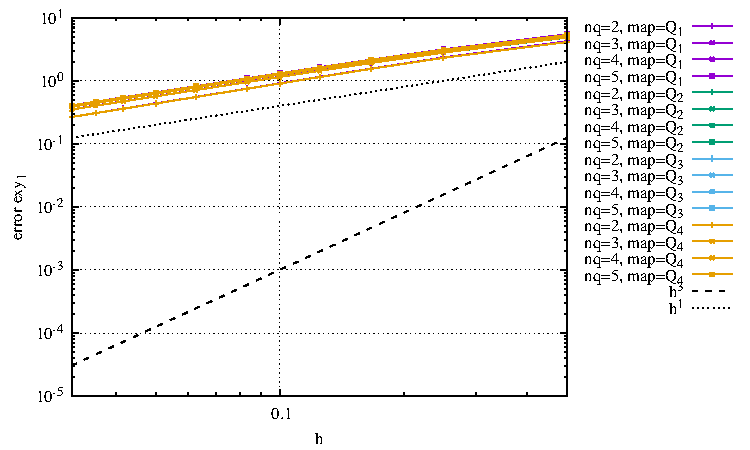
\includegraphics[width=5.7cm]{python_codes/fieldstone_152/results/exp0/err_exy1}\\
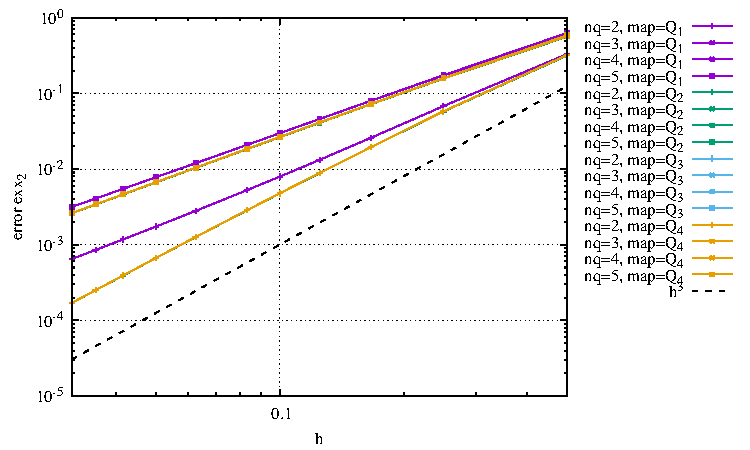
\includegraphics[width=5.7cm]{python_codes/fieldstone_152/results/exp0/err_exx2}
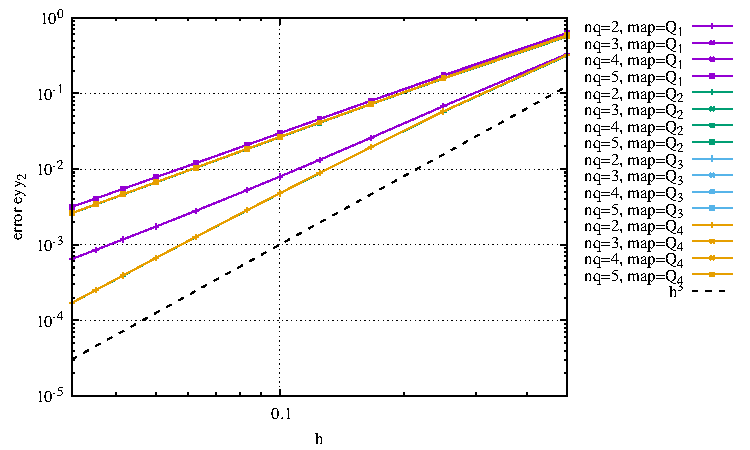
\includegraphics[width=5.7cm]{python_codes/fieldstone_152/results/exp0/err_eyy2}
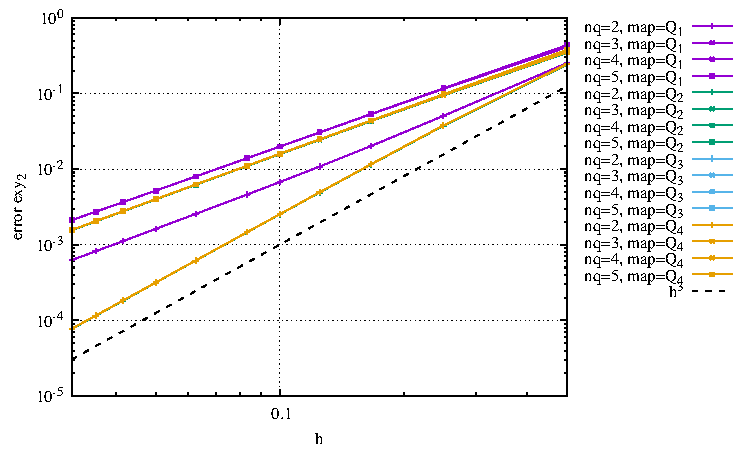
\includegraphics[width=5.7cm]{python_codes/fieldstone_152/results/exp0/err_exy2}\\
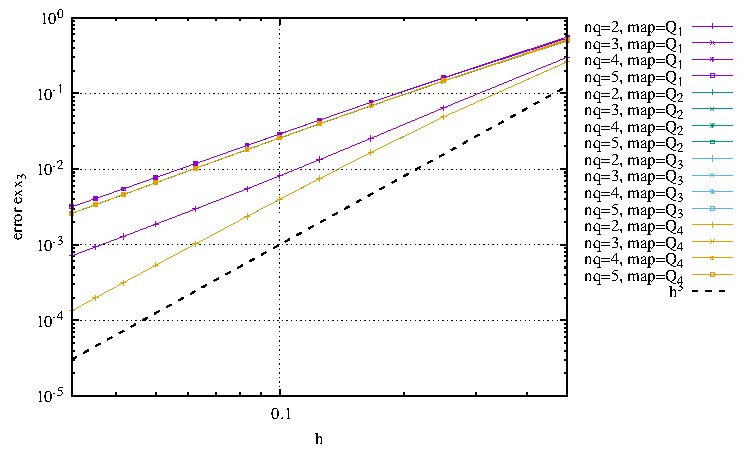
\includegraphics[width=5.7cm]{python_codes/fieldstone_152/results/exp0/err_exx3}
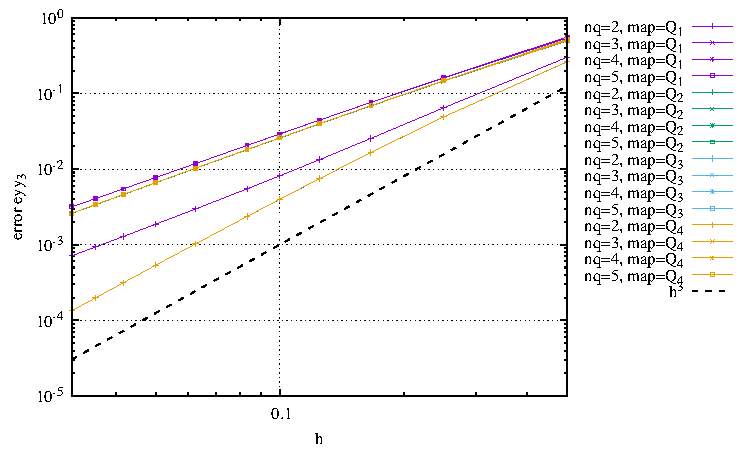
\includegraphics[width=5.7cm]{python_codes/fieldstone_152/results/exp0/err_eyy3}
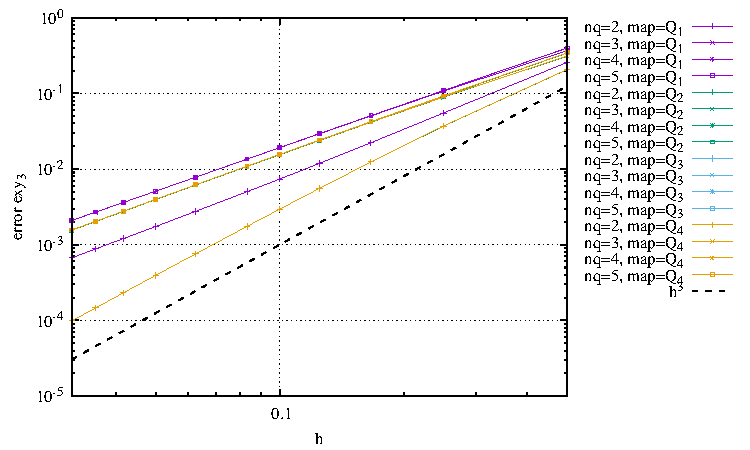
\includegraphics[width=5.7cm]{python_codes/fieldstone_152/results/exp0/err_exy3}
\end{center}

Why the super-convergence for nqperdim=2 ?!?



\newpage
%%%%%%%%%%%%%%%%%%%%%%%%%%%%%%%%%%%%%%%%%%%%%%%%%%%%%%%%%%%%%%%%%%%%%%%%%%%%%%%%%%%%%
\section*{The aquarium test (exp=1) - plane strain}

\begin{lstlisting}
axisymmetric=False
exp=1
surface_free_slip=True
\end{lstlisting}

\begin{center}
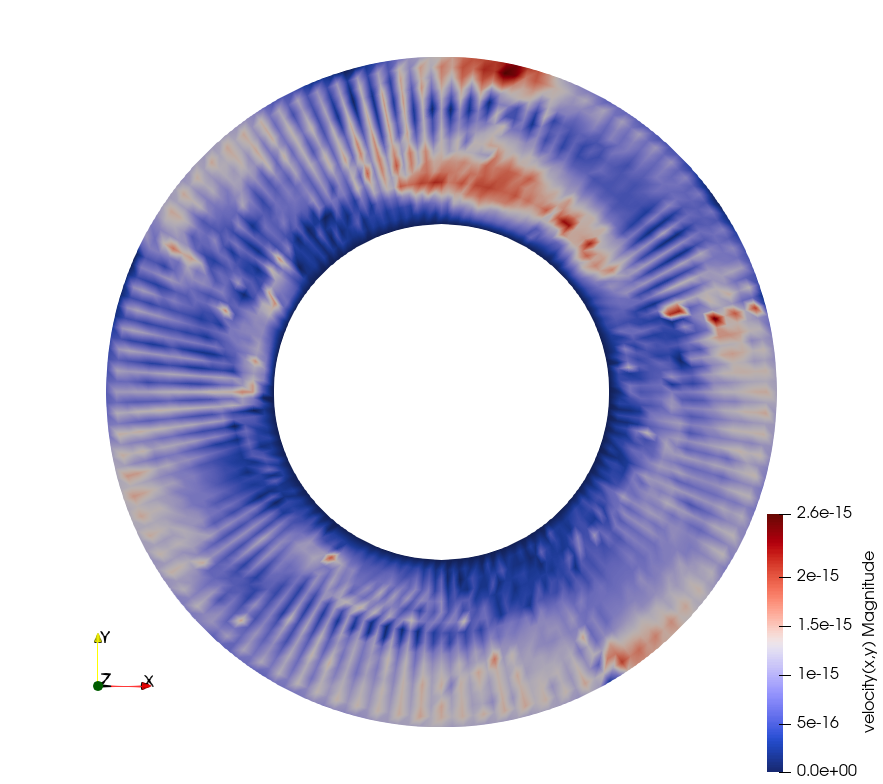
\includegraphics[width=5cm]{python_codes/fieldstone_152/results/exp1/vel}
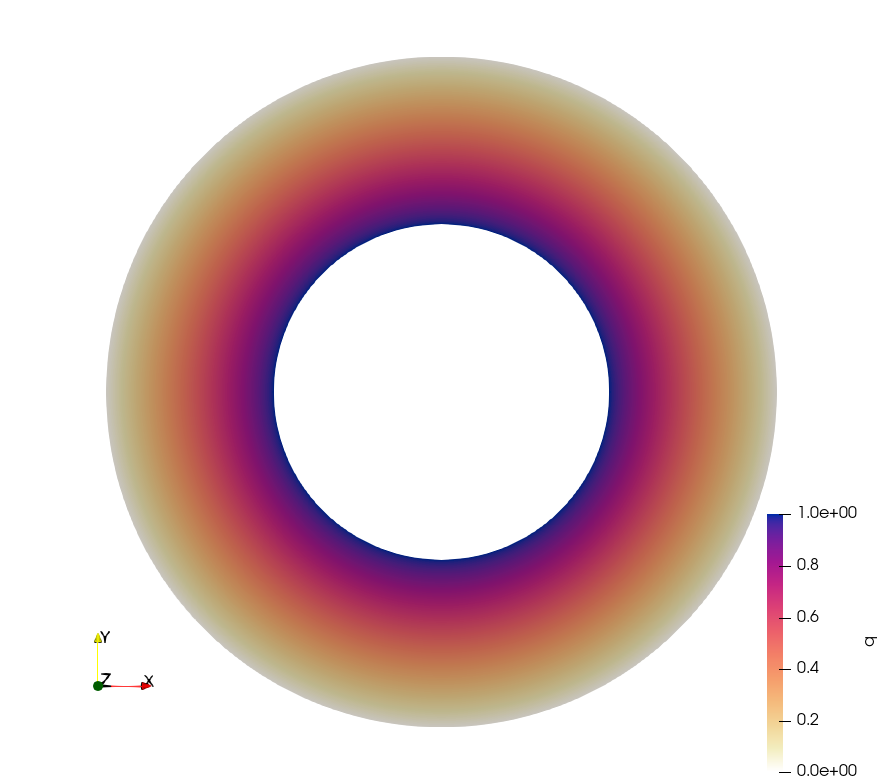
\includegraphics[width=5cm]{python_codes/fieldstone_152/results/exp1/press}\\
{\captionfont Obtained with Q4 mapping and nqperdim=3.}
\end{center}

\begin{center}
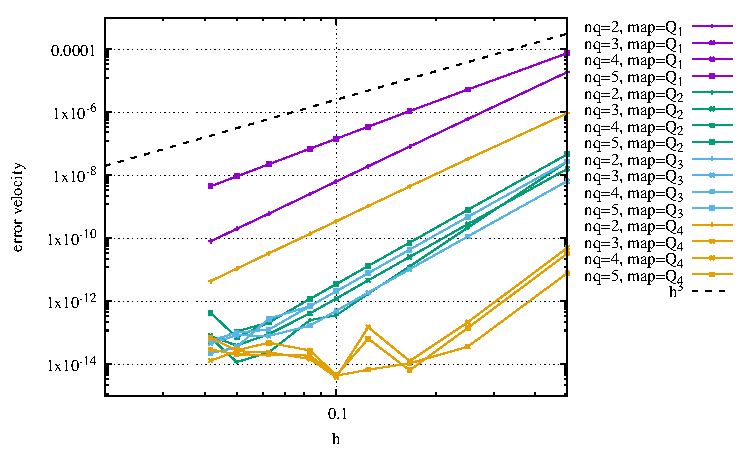
\includegraphics[width=8.3cm]{python_codes/fieldstone_152/results/exp1/errv}
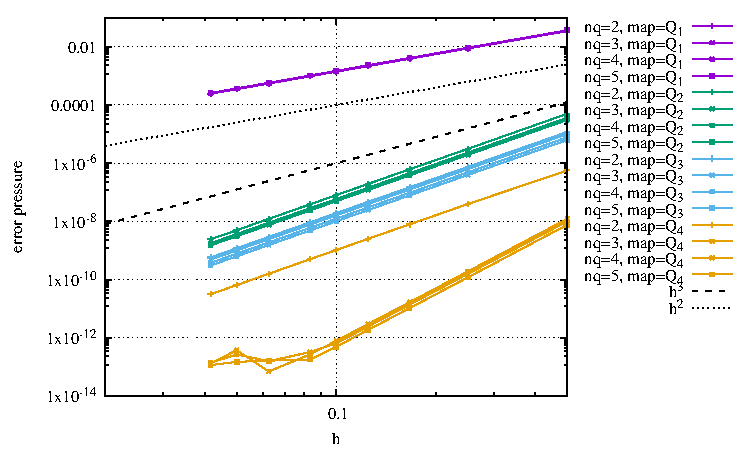
\includegraphics[width=8.3cm]{python_codes/fieldstone_152/results/exp1/errp}\\
{\captionfont Obtained with {\tt script\_errors}.}
\end{center}

\begin{center}
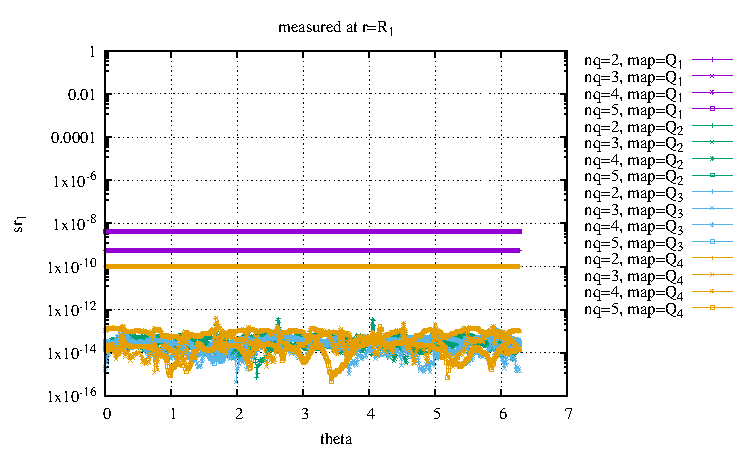
\includegraphics[width=5.7cm]{python_codes/fieldstone_152/results/exp1/sr1_R1}
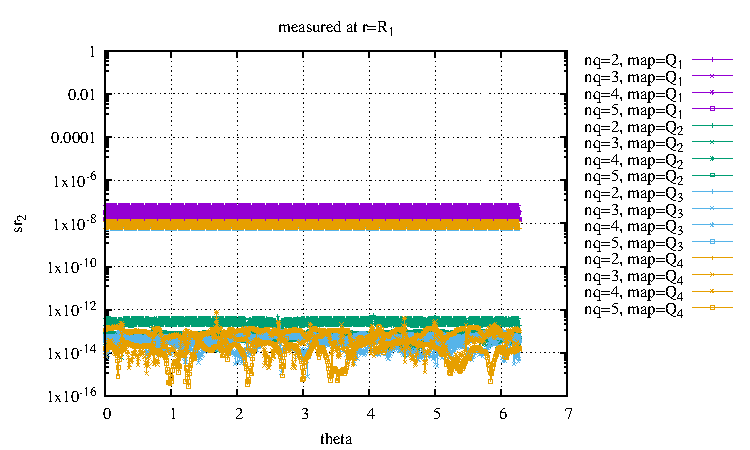
\includegraphics[width=5.7cm]{python_codes/fieldstone_152/results/exp1/sr2_R1}
\includegraphics[width=5.7cm]{python_codes/fieldstone_152/results/exp1/sr3_R1}\\
\includegraphics[width=8.3cm]{python_codes/fieldstone_152/results/exp1/sr1_R2}
\includegraphics[width=8.3cm]{python_codes/fieldstone_152/results/exp1/sr2_R2}\\
\includegraphics[width=8.3cm]{python_codes/fieldstone_152/results/exp1/sr3_R2}
\includegraphics[width=8.3cm]{python_codes/fieldstone_152/results/exp1/src_R2}\\
\includegraphics[width=8.3cm]{python_codes/fieldstone_152/results/exp1/qqq_R1}
\includegraphics[width=8.3cm]{python_codes/fieldstone_152/results/exp1/qqq_R2}\\
\includegraphics[width=8.3cm]{python_codes/fieldstone_152/results/exp1/vel_R2}
\includegraphics[width=8.3cm]{python_codes/fieldstone_152/results/exp1/err_R2}\\
{\captionfont Obtained with 32x elements. Obtained with {\tt script\_sr}.}
\end{center}


\newpage
%%%%%%%%%%%%%%%%%%%%%%%%%%%%%%%%%%%%%%%%%%%%%%%%%%%%%%%%%%%%%%%%%%%%%%%%%%%%%%%%%%%%%
\section*{The aquarium test (exp=1) - axisymmetric}

\begin{lstlisting}
axisymmetric=True
exp=1
surface_free_slip=True
\end{lstlisting}



\begin{center}
\includegraphics[width=8.3cm]{python_codes/fieldstone_152/results/exp1_axisymmetric/errv}
\includegraphics[width=8.3cm]{python_codes/fieldstone_152/results/exp1_axisymmetric/errp}
\end{center}


\begin{center}
\includegraphics[width=5.7cm]{python_codes/fieldstone_152/results/exp1_axisymmetric/sr1_R1}
\includegraphics[width=5.7cm]{python_codes/fieldstone_152/results/exp1_axisymmetric/sr2_R1}
\includegraphics[width=5.7cm]{python_codes/fieldstone_152/results/exp1_axisymmetric/sr3_R1}\\
\includegraphics[width=8.3cm]{python_codes/fieldstone_152/results/exp1_axisymmetric/sr1_R2}
\includegraphics[width=8.3cm]{python_codes/fieldstone_152/results/exp1_axisymmetric/sr2_R2}\\
\includegraphics[width=8.3cm]{python_codes/fieldstone_152/results/exp1_axisymmetric/sr3_R2}
\includegraphics[width=8.3cm]{python_codes/fieldstone_152/results/exp1_axisymmetric/src_R2}\\
\includegraphics[width=8.3cm]{python_codes/fieldstone_152/results/exp1_axisymmetric/qqq_R1}
\includegraphics[width=8.3cm]{python_codes/fieldstone_152/results/exp1_axisymmetric/qqq_R2}\\
\includegraphics[width=8.3cm]{python_codes/fieldstone_152/results/exp1_axisymmetric/vel_R2}
\includegraphics[width=8.3cm]{python_codes/fieldstone_152/results/exp1_axisymmetric/err_R2}\\
{\captionfont Obtained with 32x elements. Obtained with {\tt script\_sr}.}
\end{center}

Conclusion: best/cheapest results obtained for nqperdim=4 and Q4



\newpage
%%%%%%%%%%%%%%%%%%%%%%%%%%%%%%%%%%%%%%%%%%%%%%%%%%%%%%%%%%%%%%%%%%%%%%%%%%%%%%%%%%%%%
\section*{The blob test (exp=2) - plane strain}

The blob is prescribed as follows:
\begin{lstlisting}
val=rho0
if x**2+(y-1.5)**2<0.05:
   val-=0.01
\end{lstlisting}

In the light of previous results, we discard the Q1 mapping results 
and those obtained with {\python nqperdim=2}.

\begin{lstlisting}
axisymmetric=False
exp=2
surface_free_slip=True
\end{lstlisting}


\begin{center}
\includegraphics[width=5.7cm]{python_codes/fieldstone_152/results/exp2/sr1_R1}
\includegraphics[width=5.7cm]{python_codes/fieldstone_152/results/exp2/sr2_R1}
\includegraphics[width=5.7cm]{python_codes/fieldstone_152/results/exp2/sr3_R1}\\
\includegraphics[width=8.3cm]{python_codes/fieldstone_152/results/exp2/sr1_R2}
\includegraphics[width=8.3cm]{python_codes/fieldstone_152/results/exp2/sr2_R2}\\
\includegraphics[width=8.3cm]{python_codes/fieldstone_152/results/exp2/sr3_R2}
\includegraphics[width=8.3cm]{python_codes/fieldstone_152/results/exp2/src_R2}\\
\includegraphics[width=8.3cm]{python_codes/fieldstone_152/results/exp2/qqq_R1}
\includegraphics[width=8.3cm]{python_codes/fieldstone_152/results/exp2/qqq_R2}\\
\includegraphics[width=8.3cm]{python_codes/fieldstone_152/results/exp2/vel_R2}
\includegraphics[width=8.3cm]{python_codes/fieldstone_152/results/exp2/err_R2}\\
\includegraphics[width=8.3cm]{python_codes/fieldstone_152/results/exp2/d_t_R2}
\end{center}

\begin{center}
\includegraphics[width=8.3cm]{python_codes/fieldstone_152/results/exp2/aspect/meshes}
\includegraphics[width=8.3cm]{python_codes/fieldstone_152/results/exp2/aspect/rho}\\
\includegraphics[width=8.3cm]{python_codes/fieldstone_152/results/exp2/aspect/vel}
\includegraphics[width=8.3cm]{python_codes/fieldstone_152/results/exp2/aspect/press}
\end{center}

\begin{center}
\includegraphics[width=14cm]{python_codes/fieldstone_152/results/exp2/aspect/dynamic_topography.pdf}\\
{\captionfont Dynamic topography as computer with this \stone with resolution 32x... against the 
values obtained with \aspect.}
\end{center}

\newpage
%%%%%%%%%%%%%%%%%%%%%%%%%%%%%%%%%%%%%%%%%%%%%%%%%%%%%%%%%%%%%%%%%%%%%%%%%%%%%%%%%%%%%
\section*{The blob test (exp=2) - axisymmetric}

\begin{lstlisting}
axisymmetric=True
exp=2
surface_free_slip=True
\end{lstlisting}

\begin{center}
\includegraphics[width=5.7cm]{python_codes/fieldstone_152/results/exp2_axisymmetric/sr1_R1}
\includegraphics[width=5.7cm]{python_codes/fieldstone_152/results/exp2_axisymmetric/sr2_R1}
\includegraphics[width=5.7cm]{python_codes/fieldstone_152/results/exp2_axisymmetric/sr3_R1}\\
\includegraphics[width=8.3cm]{python_codes/fieldstone_152/results/exp2_axisymmetric/sr1_R2}
\includegraphics[width=8.3cm]{python_codes/fieldstone_152/results/exp2_axisymmetric/sr2_R2}\\
\includegraphics[width=8.3cm]{python_codes/fieldstone_152/results/exp2_axisymmetric/sr3_R2}
\includegraphics[width=8.3cm]{python_codes/fieldstone_152/results/exp2_axisymmetric/src_R2}\\
\includegraphics[width=8.3cm]{python_codes/fieldstone_152/results/exp2_axisymmetric/qqq_R1}
\includegraphics[width=8.3cm]{python_codes/fieldstone_152/results/exp2_axisymmetric/qqq_R2}\\
\includegraphics[width=8.3cm]{python_codes/fieldstone_152/results/exp2_axisymmetric/vel_R2}
\includegraphics[width=8.3cm]{python_codes/fieldstone_152/results/exp2_axisymmetric/err_R2}\\
\end{center}


\begin{center}
\includegraphics[width=12cm]{python_codes/fieldstone_152/results/exp2_axisymmetric/sr_R2_comparison}\\
{\captionfont Comparison of the effective strain rate at the surface for all three nodal methods and the 
elemental approach. Unsurprisingly the element-based strain rate is less accurate than its nodal counterpart, 
albeit smoother near the ends.}
\end{center}

\aspect models were run with the following mesh construction:
\begin{lstlisting}
subsection Mesh refinement
  set Initial global refinement          = 4 #3
  set Initial adaptive refinement        = 3 #2
  set Refinement fraction                = 0.5
  set Coarsening fraction                = 0.
  set Strategy                           = composition, strain rate
end
\end{lstlisting}


\begin{center}
\includegraphics[width=8cm]{python_codes/fieldstone_152/results/exp2_axisymmetric/aspect/dynamic_topography.pdf}
\includegraphics[width=8cm]{python_codes/fieldstone_152/results/exp2_axisymmetric/aspect/dynamic_topography_zoom.pdf}\\
{\captionfont Dynamic topography as computer with this \stone with resolution 32x... against the 
values obtained with \aspect.}
\end{center}

\begin{center}
\includegraphics[width=8cm]{python_codes/fieldstone_152/results/exp2_axisymmetric/aspect/mesh}
\includegraphics[width=8cm]{python_codes/fieldstone_152/results/exp2_axisymmetric/aspect/mesh2}\\
{\captionfont Mesh as generated by \aspect.}
\end{center}


\begin{center}
\includegraphics[width=8cm]{python_codes/fieldstone_152/results/exp2_axisymmetric/aspect/vel}
\includegraphics[width=8cm]{python_codes/fieldstone_152/results/exp2_axisymmetric/aspect/press}\\
\includegraphics[width=8cm]{python_codes/fieldstone_152/results/exp2_axisymmetric/aspect/vr}
\includegraphics[width=8cm]{python_codes/fieldstone_152/results/exp2_axisymmetric/aspect/vphi}\\
\includegraphics[width=8cm]{python_codes/fieldstone_152/results/exp2_axisymmetric/aspect/eyy}
\includegraphics[width=8cm]{python_codes/fieldstone_152/results/exp2_axisymmetric/aspect/exy}\\
\includegraphics[width=8cm]{python_codes/fieldstone_152/results/exp2_axisymmetric/aspect/sr}
\includegraphics[width=8cm]{python_codes/fieldstone_152/results/exp2_axisymmetric/aspect/sr2}\\
{\captionfont Left half of annulus is \aspect, right half is this \stone. 
We find that the strain rate field as obtained with \aspect with a reasonably high 
resolution still highlights the underlying mesh. As such we can't really compare our axisymmetric 
results with those of \aspect. Note that since this \stone computes the solution in the 
$x,y$-plane the vtu file had to be rotated so as to align with the vtu file returned by \aspect.}
\end{center}

\begin{center}
\includegraphics[width=8cm]{python_codes/fieldstone_152/results/exp2_axisymmetric/aspect/sols}
\end{center}





\newpage
%%%%%%%%%%%%%%%%%%%%%%%%%%%%%%%%%%%%%%%%%%%%%%%%%%%%%%%%%%%%%%%%%%%%%%%%%%%%%%%%%%%%%%%%%%%%%%%%%%%
\par\noindent\rule{\textwidth}{0.4pt}

%\vspace{.5cm}
%\begin{center}
%\fbox{\begin{minipage}{0.9\textwidth}
%{\color{teal}To Do, open questions, future work?}
%\begin{itemize}
%\item do smthg
%\end{itemize}
%\end{minipage}}
%\end{center}

%%%%%%%%%%%%%%%%%%%%%%%%%%%%%%%%%%%%%%%%%%%%%%%%%%%%%%%%%%%%%%%%%%%%%%%%%%%%%%%%%%%%%%%%%%%%%%%%%%%
\vspace{.5cm}

\noindent\Literature:\\
\fullcite{zizh92a}\\
\fullcite{zizh92b}


